\chapter{Technical details for Bayesian quantile deep echo state networks}
\label{app:qdesn-technical}

This appendix preserves the detailed derivations, algorithms, and
secondary diagnostics supporting the corresponding research chapter.
The chapter retains the inferential target, central model, principal
evidence, interpretation, and limitations needed for a continuous read.

% migration-id: MIG-CH04-01
\section{Shared distributional conventions}
\label{qdesn:sec:dist_conventions}

\noindent\textbf{Shared parameterizations.}
The posterior kernels below use the following distributional
parameterizations. These conventions are used in the MCMC,
coordinate-ascent variational inference (CAVI), and evidence lower bound (ELBO)
derivations below; in particular, all inverse-gamma distributions use a rate in
the reciprocal scale.

The inverse-gamma (IG) parameterization is
\[
p(x\mid a,b)=\frac{b^a}{\Gamma(a)}x^{-a-1}\exp(-b/x),\qquad x>0,
\]
and the generalized inverse Gaussian (GIG) parameterization
\[
p(x\mid \lambda,\chi,\psi)
\propto x^{\lambda-1}\exp\left\{-\frac12(\chi/x+\psi x)\right\},
\qquad x>0.
\]
The notation \(\TN(m,V)\) denotes a Normal distribution with mean \(m\) and
variance \(V\), truncated to \((0,\infty)\). The functions \(\Phi\) and
\(\phi\) denote the standard Normal distribution and density functions. The
notation \(\StudentT_\nu(\vect m,\mat S)\) denotes a multivariate Student
\(t\) distribution with degrees of freedom \(\nu\), location \(\vect m\), and
scale matrix \(\mat S\); its covariance is
\(\nu(\nu-2)^{-1}\mat S\) when \(\nu>2\).

\noindent\textbf{AL constants.}
For a fixed target quantile \(p_0\in(0,1)\), the AL constants are
\[
A_0=\frac{1-2p_0}{p_0(1-p_0)},\qquad
B_0=\frac{2}{p_0(1-p_0)}.
\]
\noindent\textbf{exAL branch constants.}
The notation \(\exAL\) denotes the quantile-fixed generalized asymmetric
Laplace distribution of \citet{exd-yan2025family}. This convention emphasizes the
role of the likelihood as an extension of AL while preserving the
quantile-fixed parameterization that identifies \(\mu\) as the target
conditional quantile. The exAL likelihood
introduces an asymmetry parameter \(\gamma\in(L,U)\), where \(L\) and
\(U\) are determined by the quantile-identifying construction. Define
\[
g(\gamma)=2\Phi(-|\gamma|)\exp(\gamma^2/2),\qquad
p_\gamma=\ind\{\gamma<0\}
+\frac{p_0-\ind\{\gamma<0\}}{g(\gamma)}.
\]
Then, with the fixed probability level shown explicitly when needed,
\[
\begin{alignedat}{2}
A_{p_0}(\gamma)\equiv A_\gamma
&=\frac{1-2p_\gamma}{p_\gamma(1-p_\gamma)},
&\qquad B_{p_0}(\gamma)\equiv B_\gamma
&=\frac{2}{p_\gamma(1-p_\gamma)},\\
C_\gamma&=\{\ind\{\gamma>0\}-p_\gamma\}^{-1},
& D_\gamma\equiv D_{p_0}(\gamma)&=C_\gamma|\gamma|.
\end{alignedat}
\]
The shorthand \(D_\gamma\) reduces visual clutter in posterior kernels and is
distinct from the regularized-horseshoe local scales \(\lambda_j\).

\noindent\textbf{AL nesting and branchwise regularity.}
When \(\gamma=0\) and the \(s_t\) latents are omitted, the exAL hierarchy
reduces to the AL working likelihood with constants \(A_0,B_0\).
This nesting is exact. The surrounding \(p_\gamma\), \(A_\gamma\),
\(B_\gamma\), and \(D_\gamma\) maps are branchwise smooth for
\(\gamma<0\) and \(\gamma>0\), but the absolute value and indicator branches
make generic two-sided derivative statements at \(\gamma=0\) invalid except in
special symmetric cases. In particular, the one-sided derivatives of
\(p_\gamma\) at zero are proportional to \(1-p_0\) from the left and to
\(p_0\) from the right. At \(\gamma=0\), calculations use the nested AL model;
for \(\gamma\ne0\), numerical derivatives are evaluated within the
corresponding sign region.

\section{Q--DESN working likelihoods, priors, and augmented posterior}
\label{qdesn:sec:model_joint}

The augmented posterior densities below are used by both computational
schemes. The AL and exAL likelihoods are working likelihoods for a
fixed target quantile, while the auxiliary variables provide equivalent
mixture representations for computation.

\section{AL and exAL augmented likelihoods}

The exAL Q--DESN observation hierarchy is
\begin{align}
v_t\mid\sigma &\sim \Exp(\text{rate}=1/\sigma),&
s_t&\sim\TN(0,1),\\
y_t\mid\vect\beta,\sigma,\gamma,v_t,s_t,\mat X
&\sim
\Normal\left(
\vect x_t^\top\vect\beta+\sigma D_\gamma s_t+A_\gamma v_t,
\sigma B_\gamma v_t
\right).
\label{qdesn:eq:supp_exal_hierarchy}
\end{align}
The marginal \(p_0\)-quantile of \(y_t\mid\vect x_t\) is
\(\vect x_t^\top\vect\beta\). The AL special case is
\begin{align}
v_t\mid\sigma &\sim \Exp(\text{rate}=1/\sigma),\\
y_t\mid\vect\beta,\sigma,v_t,\mat X
&\sim
\Normal\left(
\vect x_t^\top\vect\beta+A_0v_t,
\sigma B_0v_t
\right).
\label{qdesn:eq:supp_al_hierarchy}
\end{align}

\section{Coefficient priors}
\label{qdesn:sec:priors}

The coefficient prior regularizes the high-dimensional regression after the
reservoir features have been fixed. The ridge prior is the default Gaussian
baseline. The regularized-horseshoe prior is the adaptive global-local shrinkage
alternative; its product representation keeps the local, global, and slab scale
updates in closed form.

For the ridge coefficient prior, let
\begin{equation}
\vect\beta\sim\Normal(\vect b_\beta,\mat V_\beta),
\qquad
\mat P_\beta=\mat V_\beta^{-1}.
\label{qdesn:eq:supp_ridge_prior}
\end{equation}
Applications usually keep the intercept weakly regularized and use a
diagonal slope penalty, while \eqref{qdesn:eq:supp_ridge_prior} allows a general
positive definite prior covariance.

For the regularized-horseshoe prior, the intercept is independent,
\(\beta_0\sim\Normal(b_0,V_0)\), and the non-intercept coefficients are
represented through the
Nishimura--Suchard-style regularized horseshoe construction
\citep{qdesn-CarvalhoPolsonScott2010HS,qdesn-PiironenVehtari2017RHS,exd-nishimura2023shrunken}.
For \(j=1,\ldots,r\),
\begin{equation}
p_{\mathrm{ns}}(\beta_j,\lambda_j\mid\tau,\zeta)
\propto
\exp\left(-\frac{\beta_j^2}{2\tau^2\lambda_j^2}\right)
\exp\left(-\frac{\beta_j^2}{2\zeta^2}\right)
\lambda_j^{-1}(1+\lambda_j^2)^{-1}.
\label{qdesn:eq:supp_ns_joint}
\end{equation}
Equation~\eqref{qdesn:eq:supp_ns_joint} is the marginal joint description after the
half-Cauchy auxiliary variable for the local scale has been integrated out. The
MCMC and VB derivations use the corresponding augmented product
\[
\Normal(\beta_j\mid0,\tau^2\lambda_j^2)\,
\Normal(0\mid\beta_j,\zeta^2)
\]
together with inverse-gamma auxiliaries for \(\lambda_j^2\), \(\nu_j\),
\(\tau^2\), and \(\xi\). Normalizing factors that depend on the scale
parameters are retained. This augmented product representation is the one used
in the posterior densities below.
Equivalently, the conditional coefficient law is Gaussian with effective
variance
\begin{equation}
\beta_j\mid\lambda_j,\tau,\zeta
\sim
\Normal(0,V_j),\qquad
V_j=\left(\zeta^{-2}+\tau^{-2}\lambda_j^{-2}\right)^{-1}
=\frac{\zeta^2\tau^2\lambda_j^2}{\zeta^2+\tau^2\lambda_j^2}.
\label{qdesn:eq:supp_rhs_cond_beta}
\end{equation}
Equation~\eqref{qdesn:eq:supp_rhs_cond_beta} makes the finite-slab bound explicit.
For inverse-gamma scale updates, use the half-Cauchy augmentation
\citep{qdesn-MakalicSchmidt2016SimpleSampler}:
\begin{align}
\lambda_j^2\mid\nu_j&\sim\IG(1/2,1/\nu_j),&
\nu_j&\sim\IG(1/2,1),\\
\tau^2\mid\xi&\sim\IG(1/2,1/\xi),&
\xi&\sim\IG(1/2,1/\tau_0^2),
\label{qdesn:eq:supp_hs_aux}\\
\zeta^2&\sim\IG(a_\zeta,b_\zeta),
\label{qdesn:eq:supp_zeta_prior}
\end{align}
The slab update in Eq.~\eqref{qdesn:eq:supp_zeta_prior} is omitted when
\(\zeta^2\) is fixed.

\section{Reference calibration of the global shrinkage scale}
\label{qdesn:subsec:supp-rhs-global-scale}

The hierarchy in Eq.~\eqref{qdesn:eq:supp_hs_aux} distinguishes the posterior random
global scale \(\tau\) from the fixed hyperprior scale \(\tau_0\). The latter
should reflect the response scale, the amount of information in the fitting
sample, the number of penalized coefficients, and prior information about
coefficient activity. We first state the Gaussian reference calculation of
\citet{qdesn-PiironenVehtari2017RHS} and then describe its use for Q--DESN.

Let \(N_{\mathrm{fit}}\) be the number of fitting observations, let \(r\) be
the number of standardized non-intercept columns, and let
\(\sigma_{\mathrm{ref}}>0\) be a residual-scale reference. Under an orthogonal
Gaussian design, the ordinary-horseshoe shrinkage factor for coefficient \(j\)
is
\begin{equation}
\kappa_j
=\left(1+
\frac{N_{\mathrm{fit}}\tau^2\lambda_j^2}
{\sigma_{\mathrm{ref}}^2}
\right)^{-1}.
\label{qdesn:eq:supp-rhs-kappa-reference}
\end{equation}
If
\(m_{\mathrm{eff}}=\sum_{j=1}^r(1-\kappa_j)\), integration over the
half-Cauchy local scales gives
\begin{equation}
\E(m_{\mathrm{eff}}\mid\tau,\sigma_{\mathrm{ref}})
=r\frac{a}{1+a},
\qquad
a=\frac{\tau\sqrt{N_{\mathrm{fit}}}}{\sigma_{\mathrm{ref}}}.
\label{qdesn:eq:supp-rhs-effective-size-reference}
\end{equation}
Equating Eq.~\eqref{qdesn:eq:supp-rhs-effective-size-reference} to an elicited prior
reference \(m_0\in(0,r)\) and using the resulting scale for the half-Cauchy
hyperprior gives
\begin{equation}
\tau_{0,\mathrm{ref}}
=\frac{m_0}{r-m_0}
 \frac{\sigma_{\mathrm{ref}}}{\sqrt{N_{\mathrm{fit}}}}.
\label{qdesn:eq:supp-rhs-tau0-gaussian-reference}
\end{equation}
Here \(m_0\) represents prior information about the number of coefficients
expected to escape strong global shrinkage; it is not a model size selected by
validation. When both the response and the penalized columns are standardized
using the fitting observations, setting \(\sigma_{\mathrm{ref}}=1\) gives the
unit-scale version of Eq.~\eqref{qdesn:eq:supp-rhs-tau0-gaussian-reference}. If only
the design columns are standardized, \(\sigma_{\mathrm{ref}}\) should remain
on the response scale and may be obtained from the preliminary Gaussian fit.

Equations~\eqref{qdesn:eq:supp-rhs-kappa-reference}--%
\eqref{qdesn:eq:supp-rhs-tau0-gaussian-reference} give an exact effective-size
relationship for the ordinary horseshoe under the stated orthogonal Gaussian
reference. They are not an exact effective-size identity for the prior in
Eq.~\eqref{qdesn:eq:supp_ns_joint}. In particular, the finite slab changes the
coefficient variance when a local scale is large, and the DESN design can be
strongly correlated. We therefore use
Eq.~\eqref{qdesn:eq:supp-rhs-tau0-gaussian-reference} as an interpretable reference
calibration for the Nishimura--Suchard construction, not as a guarantee that
the posterior contains exactly \(m_0\) active coefficients.

\noindent\textbf{Likelihood-information alternatives.}
A likelihood-specific reference can be obtained by replacing the Gaussian
location information with the information under the working likelihood. Let
\(I_{\mu,\mathrm{ref}}\) be the one-observation Fisher information for the
location parameter at a specified reference state. The corresponding local
information match is
\begin{equation}
\tau_{0,f}
=\frac{m_0}{r-m_0}
 \{N_{\mathrm{fit}}I_{\mu,\mathrm{ref}}\}^{-1/2}.
\label{qdesn:eq:supp-rhs-tau0-information-reference}
\end{equation}
For the AL density at probability level \(p_0\), the location score equals
\(\{p_0-\ind(y<\mu)\}/\sigma\) except at \(y=\mu\), an event of probability
zero under the continuous working likelihood. Hence
\begin{equation}
I_{\mu,\mathrm{AL}}
=\frac{p_0(1-p_0)}{\sigma^2},
\qquad
\tau_{0,\mathrm{AL},p_0}
=\frac{m_0}{r-m_0}
 \frac{\sigma_{\mathrm{ref},p_0}}
 {\sqrt{N_{\mathrm{fit}}p_0(1-p_0)}}.
\label{qdesn:eq:supp-rhs-tau0-al-reference}
\end{equation}
For the exAL likelihood, write the standardized density as
\(g_{p_0}(z;\gamma)\), where \(z=(y-\mu)/\sigma\), and define
\begin{equation}
J_{p_0}(\gamma)
=\E\left[
\left\{\frac{\partial}{\partial z}
\log g_{p_0}(Z;\gamma)\right\}^{2}
\right].
\label{qdesn:eq:supp-exal-standardized-location-information}
\end{equation}
Equation~\eqref{qdesn:eq:supp-exal-standardized-location-information} implies
\(I_{\mu,\mathrm{exAL}}=J_{p_0}(\gamma)/\sigma^2\), which gives
\begin{equation}
\tau_{0,\mathrm{exAL},p_0}
=\frac{m_0}{r-m_0}
 \frac{\sigma_{\mathrm{ref},p_0}}
 {\sqrt{N_{\mathrm{fit}}J_{p_0}(\gamma_{\mathrm{ref}})}}.
\label{qdesn:eq:supp-rhs-tau0-exal-reference}
\end{equation}
At the nested AL reference \(\gamma_{\mathrm{ref}}=0\),
\(J_{p_0}(0)=p_0(1-p_0)\), so
Eq.~\eqref{qdesn:eq:supp-rhs-tau0-exal-reference} reduces to
Eq.~\eqref{qdesn:eq:supp-rhs-tau0-al-reference}. These information-based scales are
local reference calculations under the working likelihoods. They do not
correct likelihood misspecification or establish frequentist calibration.
Equation~\eqref{qdesn:eq:supp-rhs-tau0-information-reference} uses equally weighted
likelihood contributions. For a weighted or composite likelihood, the
corresponding reference should use the total expected location curvature of
the stated likelihood rather than substituting its raw number of rows for
\(N_{\mathrm{fit}}\).

\noindent\textbf{Recommendation for the model sequence.}
When the preliminary Gaussian, AL, and exAL regressions use the same
standardized design, the common value in
Eq.~\eqref{qdesn:eq:supp-rhs-tau0-gaussian-reference} is the preferred default for
comparing the likelihood families. It holds the coefficient-prior scale fixed
while each model retains its own likelihood and posterior. The AL and exAL
information references are useful sensitivity specifications when
likelihood-specific curvature matching is the scientific objective.

For joint quantile regressions, the baseline slope and adjacent-difference
blocks may be calibrated separately. An elicited value \(m_0^0\) applies to
the baseline coefficients, while values \(m_{0,k}^{\Delta}\) apply to the
adjacent differences. Choosing smaller \(m_{0,k}^{\Delta}\) expresses a
stronger prior belief that neighboring quantile levels have similar slopes.
Likewise, application models with distinct reference-process and discrepancy
designs should calibrate those blocks separately when their dimensions,
standardizations, or prior activity beliefs differ.

A reproducible specification therefore records
\(N_{\mathrm{fit}}\), \(r\), \(m_0\), \(\sigma_{\mathrm{ref}}\), the
observations used for standardization, and whether the Gaussian or a
likelihood-information reference was used. Sequential initialization changes
only numerical starting values and does not change this prior specification.

\section{Augmented posterior densities}

\noindent\textbf{Augmented-posterior convention.}
Each AL or exAL mixture variable appears once. Inverse-gamma variables augment
only the shrinkage scales. Let \(f\in\{\mathrm{AL},\mathrm{exAL}\}\), let
\(\vect a_f=\vect v\) for AL and
\(\vect a_f=(\vect v^\top,\vect s^\top)^\top\) for exAL, and let
\(\eta_f\) be empty for AL and equal to \(\gamma\) for exAL. The common
augmented target is
\begin{equation}
\begin{aligned}
&p(\vect y,\vect a_f,\vect\beta,\sigma,\eta_f,
\Theta_h\mid\mat X)\\
&\quad\propto
\prod_{t=1}^T
p_f(y_t\mid\vect\beta,\sigma,\eta_f,\vect a_{f,t},\vect x_t)
p_f(\vect a_{f,t}\mid\sigma)\,
p_h(\vect\beta,\Theta_h)\,p(\sigma)\,p_f(\eta_f),
\end{aligned}
\label{qdesn:eq:supp-generic-augmented-target}
\end{equation}
where \(h\in\{\mathrm{ridge},\mathrm{RHS}\}\). For ridge,
\(\Theta_h\) is empty and \(p_h(\vect\beta,\Theta_h)\) is
Eq.~\eqref{qdesn:eq:supp_ridge_prior}. For RHS,
\(\Theta_h=(\vect\lambda^2,\vect\nu,\tau^2,\xi,\zeta^2)\), and
\(p_h\) is the product of the intercept prior, the Gaussian product in
Eq.~\eqref{qdesn:eq:supp_ns_joint}, and the scale priors in
Eq.~\eqref{qdesn:eq:supp_hs_aux}. The AL factor uses
Eq.~\eqref{qdesn:eq:supp_al_hierarchy}; its \(p_f(\eta_f)\) factor is one. The exAL
factor uses Eq.~\eqref{qdesn:eq:supp_exal_hierarchy}, includes \(p(s_t)\), and has
\(p_f(\eta_f)=\pi_\gamma(\gamma)\ind\{L<\gamma<U\}\). Viewed as a function
of the unknown quantities conditional on \((\vect y,\mat X)\),
Eq.~\eqref{qdesn:eq:supp-generic-augmented-target} defines the four posterior
targets without repeating blocks that differ only by omission.

\section{Gaussian DESN baseline and initialization}
\label{qdesn:gauss:sec:scope}

After reservoir construction, spectral scaling, layer reduction, and washout,
the DESN feature map is fixed. Posterior inference for the readout is therefore
conditional on a deterministic design matrix
\(\mat X=[\vect x_1^\top;\ldots;\vect x_T^\top]\). The Gaussian DESN considered
in this section replaces the AL or exAL working likelihood with the homoskedastic
Normal likelihood
\begin{equation}
\label{qdesn:gauss:eq:gaussian_likelihood_scope}
\vect y\mid \vect\beta,\omega^2,\mat X
\sim \Normal_T(\mat X\vect\beta,\omega^2\mat I_T),
\qquad \omega^2>0.
\end{equation}
The variance parameter is denoted by \(\omega^2\), not \(\sigma\), to avoid
confusion with the AL/exAL scale parameter in Q--DESN.

The Gaussian DESN is not a quantile model. If the Gaussian likelihood is taken
literally, \(\vect x_t^\top\vect\beta\) targets a conditional mean under
squared-error loss. In Q--DESN, by contrast, \(\vect x_t^\top\vect\beta\) is the
conditional \(p_0\)-quantile under an AL or exAL working likelihood. Its role
is therefore computational:
\begin{enumerate}[label=(\roman*)]
\item provide an exact mean-regression baseline on the same fixed DESN features;
\item provide a conditioning and regularization diagnostic for the readout;
\item provide stable initial values for AL and exAL Q--DESN algorithms;
\item avoid unnecessary approximate inference for a model whose posterior is
available analytically.
\end{enumerate}

\section{Fixed design and notation}
\label{qdesn:gauss:sec:fixed_design}

Let
\begin{equation}
\label{qdesn:gauss:eq:y_X_beta_dimensions}
\vect y=(y_1,\ldots,y_T)^\top\in\R^T,
\qquad
\mat X=[\vect x_1^\top;\ldots;\vect x_T^\top]\in\R^{T\times d},
\qquad d=r+1.
\end{equation}
Each row vector \(\vect x_t=(1,\tilde{\vect x}_t^\top)^\top\in\R^d\) contains
an intercept and \(r\) fixed DESN readout features. The coefficient vector is
partitioned as
\begin{equation}
\label{qdesn:gauss:eq:beta_partition}
\vect\beta=(\beta_0,\beta_1,\ldots,\beta_r)^\top\in\R^d,
\qquad
\vect\beta_{1:r}=(\beta_1,\ldots,\beta_r)^\top.
\end{equation}
The first coefficient is the intercept. The remaining \(r\) coefficients are
slopes associated with the fixed DESN features. No reservoir weight, input
weight, reducer, leak rate, or spectral-radius parameter is inferred in this
Gaussian readout.

For any \(\vect\beta\), define
\begin{equation}
\label{qdesn:gauss:eq:residuals}
\vect e(\vect\beta)=\vect y-\mat X\vect\beta,
\qquad
S_y(\vect\beta)=\|\vect y-\mat X\vect\beta\|^2.
\end{equation}
The identity matrix of size \(m\) is \(\mat I_m\).

\section{Exact scaled-ridge model and posterior}
\label{qdesn:gauss:sec:scaled_ridge}

\subsection{Model}
\label{qdesn:gauss:subsec:model}

The exact Gaussian baseline uses the conjugate scaled ridge prior
\begin{align}
\vect y\mid\vect\beta,\omega^2,\mat X
&\sim \Normal_T(\mat X\vect\beta,\omega^2\mat I_T),
\label{qdesn:gauss:eq:likelihood}\\
\vect\beta\mid\omega^2
&\sim \Normal_d(\vect b,\omega^2\mat P^{-1}),
\label{qdesn:gauss:eq:scaled_prior}\\
\omega^2&\sim\IG(a_\omega,b_\omega),
\label{qdesn:gauss:eq:omega_prior}
\end{align}
where \(a_\omega,b_\omega>0\), \(\mat P\in\R^{d\times d}\) is positive
definite, and
\begin{equation}
\label{qdesn:gauss:eq:b_P_definition}
\vect b=(b_0,0,\ldots,0)^\top,
\qquad
\mat P=\diag(P_0,\kappa_\beta^{-2},\ldots,\kappa_\beta^{-2}).
\end{equation}
If
\(\beta_0\mid\omega^2\sim\Normal(b_0,\omega^2V_0)\), then
\(P_0=V_0^{-1}\). More general positive definite \(\mat P\) can be used without
changing the derivation.

The scaling by \(\omega^2\) in \eqref{qdesn:gauss:eq:scaled_prior} is the key conjugacy
condition. It is not identical to an independent ridge prior
\(\vect\beta\sim\Normal_d(\vect b,\mat P^{-1})\). The scaled version is retained
here because it yields an exact one-shot posterior and is used only as a
baseline and initialization device for Q--DESN.

\subsection{Full joint distribution}
\label{qdesn:gauss:subsec:joint}

The joint density factors as
\begin{equation}
\label{qdesn:gauss:eq:joint_factorization}
p(\vect y,\vect\beta,\omega^2\mid\mat X)
=p(\vect y\mid\vect\beta,\omega^2,\mat X)
 p(\vect\beta\mid\omega^2)p(\omega^2).
\end{equation}
Writing all terms that depend on unknowns,
\begin{align}
\label{qdesn:gauss:eq:joint_density_explicit}
p(\vect y,\vect\beta,\omega^2\mid\mat X)
&=(2\pi\omega^2)^{-T/2}
\exp\left\{-\frac{1}{2\omega^2}
(\vect y-\mat X\vect\beta)^\top(\vect y-\mat X\vect\beta)\right\}
\nonumber\\
&\quad\times
(2\pi\omega^2)^{-d/2}|\mat P|^{1/2}
\exp\left\{-\frac{1}{2\omega^2}
(\vect\beta-\vect b)^\top\mat P(\vect\beta-\vect b)\right\}
\nonumber\\
&\quad\times
\frac{b_\omega^{a_\omega}}{\Gamma(a_\omega)}
(\omega^2)^{-a_\omega-1}\exp(-b_\omega/\omega^2).
\end{align}
Equivalently, up to constants independent of \((\vect\beta,\omega^2)\),
\begin{align}
\label{qdesn:gauss:eq:log_joint}
\log p(\vect y,\vect\beta,\omega^2\mid\mat X)
&=\frac12\log|\mat P|+a_\omega\log b_\omega-\log\Gamma(a_\omega)
\nonumber\\
&\quad
-\left(a_\omega+1+\frac{T+d}{2}\right)\log\omega^2
\nonumber\\
&\quad
-\frac{1}{2\omega^2}\left[
\|\vect y-\mat X\vect\beta\|^2
+(\vect\beta-\vect b)^\top\mat P(\vect\beta-\vect b)
+2b_\omega\right].
\end{align}

\subsection{Completing the square}
\label{qdesn:gauss:subsec:complete_square}

Define
\begin{align}
\mat P_n&=\mat P+\mat X^\top\mat X,
\label{qdesn:gauss:eq:Pn}\\
\vect h_n&=\mat P\vect b+\mat X^\top\vect y,
\label{qdesn:gauss:eq:hn}\\
\vect m_n&=\mat P_n^{-1}\vect h_n,
\label{qdesn:gauss:eq:mn}\\
a_n&=a_\omega+\frac{T}{2},
\label{qdesn:gauss:eq:an}\\
B_n&=b_\omega+\frac12\left(
\vect y^\top\vect y+
\vect b^\top\mat P\vect b-
\vect m_n^\top\mat P_n\vect m_n
\right).
\label{qdesn:gauss:eq:Bn}
\end{align}
Then
\begin{align}
\label{qdesn:gauss:eq:complete_square_identity}
&\|\vect y-\mat X\vect\beta\|^2
+(\vect\beta-\vect b)^\top\mat P(\vect\beta-\vect b)
\nonumber\\
&\qquad=
(\vect\beta-\vect m_n)^\top\mat P_n(\vect\beta-\vect m_n)
+\vect y^\top\vect y+
\vect b^\top\mat P\vect b-
\vect m_n^\top\mat P_n\vect m_n.
\end{align}
Substituting \eqref{qdesn:gauss:eq:complete_square_identity} into the joint density gives
an exact Normal--inverse-gamma posterior.

\subsection{Exact posterior}
\label{qdesn:gauss:subsec:exact_posterior}

The posterior factorization is
\begin{align}
\omega^2\mid\vect y,\mat X&\sim\IG(a_n,B_n),
\label{qdesn:gauss:eq:omega_posterior}\\
\vect\beta\mid\omega^2,\vect y,\mat X
&\sim\Normal_d(\vect m_n,\omega^2\mat P_n^{-1}).
\label{qdesn:gauss:eq:beta_cond_posterior}
\end{align}
Equivalently,
\begin{equation}
\label{qdesn:gauss:eq:joint_posterior_kernel}
p(\vect\beta,\omega^2\mid\vect y,\mat X)
=p(\vect\beta\mid\omega^2,\vect y,\mat X)p(\omega^2\mid\vect y,\mat X).
\end{equation}
The marginal coefficient posterior is multivariate Student \(t\):
\begin{equation}
\label{qdesn:gauss:eq:beta_student_posterior}
\vect\beta\mid\vect y,\mat X
\sim
\StudentT_{2a_n}\left(\vect m_n,\frac{B_n}{a_n}\mat P_n^{-1}\right).
\end{equation}
Hence
\begin{align}
\E(\vect\beta\mid\vect y,\mat X)&=\vect m_n,
\label{qdesn:gauss:eq:posterior_mean_beta}\\
\Var(\vect\beta\mid\vect y,\mat X)
&=\frac{B_n}{a_n-1}\mat P_n^{-1},
\qquad a_n>1,
\label{qdesn:gauss:eq:posterior_var_beta}\\
\E(\omega^2\mid\vect y,\mat X)&=\frac{B_n}{a_n-1},
\qquad a_n>1.
\label{qdesn:gauss:eq:posterior_mean_omega}
\end{align}
The posterior mode of \(\vect\beta\) and its posterior mean coincide at
\(\vect m_n\), while the marginal posterior for \(\vect\beta\) carries the
additional uncertainty induced by integrating out \(\omega^2\).

\section{Posterior predictive distributions}
\label{qdesn:gauss:sec:predictive}

For a new fixed DESN feature vector \(\vect x_*\in\R^d\), the posterior
predictive distribution is
\begin{equation}
\label{qdesn:gauss:eq:predictive_univariate}
y_*\mid\vect y,\mat X,\vect x_*
\sim
\StudentT_{2a_n}\left(
\vect x_*^\top\vect m_n,
\frac{B_n}{a_n}\{1+\vect x_*^\top\mat P_n^{-1}\vect x_*\}
\right).
\end{equation}
More generally, for a fixed future design matrix \(\mat X_*\in\R^{H\times d}\),
\begin{equation}
\label{qdesn:gauss:eq:predictive_multivariate}
\vect y_*\mid\vect y,\mat X,\mat X_*
\sim
\StudentT_{2a_n}\left(
\mat X_*\vect m_n,
\frac{B_n}{a_n}\{\mat I_H+\mat X_*\mat P_n^{-1}\mat X_*^\top\}
\right).
\end{equation}
The fixed-design condition matters. In multi-step DESN forecasting, future
features may depend on previously simulated responses. Conditional on any
particular generated feature path, \eqref{qdesn:gauss:eq:predictive_multivariate} applies.
If the feature path is recursively simulated, posterior prediction should
propagate draws through the reservoir recursion rather than treating
\(\mat X_*\) as known in advance.

\section{Exact log marginal likelihood}
\label{qdesn:gauss:sec:log_marginal}

Integrating out both \(\vect\beta\) and \(\omega^2\) gives the closed-form
marginal likelihood
\begin{align}
\label{qdesn:gauss:eq:log_marginal}
\log p(\vect y\mid\mat X)
&=-\frac{T}{2}\log(2\pi)
+\frac12\log|\mat P|-\frac12\log|\mat P_n|
+a_\omega\log b_\omega-a_n\log B_n
\nonumber\\
&\quad+\log\Gamma(a_n)-\log\Gamma(a_\omega).
\end{align}
This replaces any need for an ELBO in the Gaussian baseline. It is also a
strong implementation check: exact posterior samplers and numerical posterior
summaries should be consistent with \eqref{qdesn:gauss:eq:log_marginal} and
\eqref{qdesn:gauss:eq:omega_posterior}--\eqref{qdesn:gauss:eq:beta_student_posterior}.

\section{Exact direct posterior sampler}
\label{qdesn:gauss:sec:direct_sampler}

Because the posterior is available exactly, no Markov chain is required.
Independent posterior draws are generated directly as follows.

\begin{algorithmblock}{Direct sampler for the exact scaled-ridge Gaussian DESN}
\label{qdesn:gauss:alg:direct_sampler}
\emph{Input:} fixed design \(\mat X\), response \(\vect y\), prior
\((\vect b,\mat P,a_\omega,b_\omega)\), and desired number of draws \(M\).
\begin{enumerate}[label=(\arabic*)]
\item Compute \(\mat P_n\), \(\vect m_n\), \(a_n\), and \(B_n\) from
\eqref{qdesn:gauss:eq:Pn}--\eqref{qdesn:gauss:eq:Bn}.
\item For \(m=1,\ldots,M\):
  \begin{enumerate}[label=(\alph*)]
  \item draw \(\omega^{2(m)}\sim\IG(a_n,B_n)\);
  \item draw
  \(\vect\beta^{(m)}\mid\omega^{2(m)}
  \sim\Normal_d(\vect m_n,\omega^{2(m)}\mat P_n^{-1})\).
  \end{enumerate}
\item For fixed future \(\mat X_*\), optionally draw
\(\vect y_*^{(m)}\sim\Normal_H(\mat X_*\vect\beta^{(m)},
\omega^{2(m)}\mat I_H)\), or use the analytic Student distribution in
\eqref{qdesn:gauss:eq:predictive_multivariate}.
\end{enumerate}
\end{algorithmblock}

Algorithm~\ref{qdesn:gauss:alg:direct_sampler} is a direct posterior sampler, not a Gibbs
sampler. A Gibbs sampler would only reproduce a posterior that is already
available in closed form. Similarly, CAVI/VB would only approximate an exact
posterior. For this reason, Gibbs, CAVI, and ELBO derivations are intentionally
omitted from the main Gaussian baseline.

\section{Initialization of AL and exAL Q--DESN}
\label{qdesn:gauss:sec:initialization}

The posterior mean \(\vect m_n\) gives a stable Gaussian readout estimate on the
same fixed DESN features used by Q--DESN. For a target quantile level
\(p_0\in(0,1)\), use it as a mean-regression warm start and then shift the
intercept to target the desired empirical quantile.

Define Gaussian residuals
\begin{equation}
\label{qdesn:gauss:eq:init_residuals}
r_t^N=y_t-\vect x_t^\top\vect m_n,
\qquad t=1,\ldots,T.
\end{equation}
Let
\begin{equation}
\label{qdesn:gauss:eq:empirical_resid_quantile}
c_{p_0}=\widehat Q_{p_0}(r_1^N,\ldots,r_T^N)
\end{equation}
be the empirical \(p_0\)-quantile of the Gaussian residuals. Set
\begin{align}
\beta_0^{\mathrm{init}}(p_0)&=m_{n,0}+c_{p_0},
\label{qdesn:gauss:eq:init_beta0}\\
\beta_j^{\mathrm{init}}(p_0)&=m_{n,j},
\qquad j=1,\ldots,r.
\label{qdesn:gauss:eq:init_betaj}
\end{align}
Then the empirical \(p_0\)-quantile of
\(y_t-\vect x_t^\top\vect\beta^{\mathrm{init}}(p_0)\) is approximately zero.
This makes \(\vect x_t^\top\vect\beta^{\mathrm{init}}(p_0)\) a more appropriate
initial quantile path than the raw Gaussian mean path.

With the check loss
\begin{equation}
\label{qdesn:gauss:eq:check_loss}
\rho_p(u)=u\{p-\ind(u<0)\},
\end{equation}
initialize the AL/exAL scale by
\begin{equation}
\label{qdesn:gauss:eq:init_sigma}
\sigma^{\mathrm{init}}
=\frac1T\sum_{t=1}^T
\rho_{p_0}\left(y_t-\vect x_t^\top\vect\beta^{\mathrm{init}}(p_0)\right)
+\epsilon,
\end{equation}
where \(\epsilon>0\) is a small numerical floor. For AL, no shape parameter or
\(s_t\) variables are used. For exAL, initialize at the AL special case,
\begin{equation}
\label{qdesn:gauss:eq:init_gamma}
\gamma^{\mathrm{init}}=0,
\end{equation}
or at a small jittered value near zero if the implementation uses an open
transformed support. Stable latent starts are
\begin{equation}
\label{qdesn:gauss:eq:init_latents}
v_t^{\mathrm{init}}=\sigma^{\mathrm{init}},
\qquad
s_t^{\mathrm{init}}=\sqrt{2/\pi}\quad\text{for exAL only}.
\end{equation}

For variational Q--DESN implementations, a Gaussian covariance scale can also
be initialized from
\begin{equation}
\label{qdesn:gauss:eq:init_covariance}
\widehat{\Var}(\vect\beta\mid\vect y,\mat X)
=\frac{B_n}{a_n-1}\mat P_n^{-1},
\qquad a_n>1,
\end{equation}
or from the conditional covariance
\(\widehat\omega^2\mat P_n^{-1}\) with
\(\widehat\omega^2=B_n/(a_n-1)\). These covariance quantities should be viewed
as numerical initializers rather than posterior uncertainty statements for the
AL/exAL quantile model.

\section{Alternative priors and scope}
\label{qdesn:gauss:sec:omitted_variants}

\subsection{Independent, unscaled ridge prior}
\label{qdesn:gauss:subsec:unscaled_omitted}

The independent ridge prior
\begin{equation}
\label{qdesn:gauss:eq:unscaled_prior_omitted}
\vect\beta\sim\Normal_d(\vect b,\mat P^{-1}),
\qquad
\omega^2\sim\IG(a_\omega,b_\omega)
\end{equation}
is conditionally conjugate: \(\vect\beta\mid\omega^2,\vect y,\mat X\) is
Gaussian and \(\omega^2\mid\vect\beta,\vect y,\mat X\) is inverse-gamma.
However, it does not yield the same one-shot Normal--inverse-gamma posterior as
Section~\ref{qdesn:gauss:sec:scaled_ridge}, because the coefficient prior is not scaled by
\(\omega^2\). It would require a Gibbs sampler or a mean-field approximation
for posterior computation. Since the purpose of this baseline is an exact Gaussian
baseline and initializer, the unscaled prior is not developed further here.

\subsection{Regularized-horseshoe readout prior}
\label{qdesn:gauss:subsec:rhs_omitted}

A Gaussian DESN with the Nishimura--Suchard regularized-horseshoe
\texttt{rhs\_ns} prior is also conditionally conjugate under its product
representation. Given the local, global, and slab scales, the coefficient block
is Gaussian, and the scale blocks can have inverse-gamma updates. Nevertheless,
after integrating over those shrinkage scales, the marginal posterior is not a
single closed-form Normal--inverse-gamma or Student distribution. Thus the
\texttt{rhs\_ns} Gaussian model is useful as a conditional Gibbs or CAVI warm
start, but it is not the exact closed-form baseline derived in this section.

For Q--DESN initialization, the recommended default is therefore
\begin{equation}
\label{qdesn:gauss:eq:init_pipeline}
\begin{gathered}
\text{exact scaled-ridge Gaussian DESN}\\
\longrightarrow\ \text{quantile-shifted }\vect\beta^{\mathrm{init}}(p_0)\\
\longrightarrow\ \text{AL/exAL Q--DESN}.
\end{gathered}
\end{equation}
If adaptive RHS shrinkage is required in the final Q--DESN fit, RHS scale
initializations can still be constructed from the shifted ridge coefficients,
for example
\begin{align}
\tau^{\mathrm{init}}
&=\operatorname{median}_{j=1,\ldots,r}|\beta_j^{\mathrm{init}}|+
\epsilon,
\label{qdesn:gauss:eq:init_tau_rhs}\\
\lambda_j^{\mathrm{init}}
&=\max\left\{\lambda_{\min},
\frac{|\beta_j^{\mathrm{init}}|}{\tau^{\mathrm{init}}}\right\},
\qquad j=1,\ldots,r,
\label{qdesn:gauss:eq:init_lambda_rhs}\\
\zeta^{\mathrm{init}}
&=\max_{j=1,\ldots,r}|\beta_j^{\mathrm{init}}|+
\epsilon.
\label{qdesn:gauss:eq:init_zeta_rhs}
\end{align}
These are initialization heuristics, not an exact RHS posterior calculation.

\section{Numerical implementation}
\label{qdesn:gauss:sec:implementation}

The main computational object is the positive definite precision matrix
\(\mat P_n=\mat P+\mat X^\top\mat X\). Implementations should use Cholesky
factorization of \(\mat P_n\) for all solves, log determinants, and Gaussian
sampling. Avoid explicit matrix inversion except in small diagnostic scripts.
For example,
\begin{equation}
\label{qdesn:gauss:eq:solve_not_inverse}
\vect m_n=\mat P_n^{-1}\vect h_n
\end{equation}
should be computed by solving \(\mat P_n\vect m_n=\vect h_n\).

For the log marginal likelihood,
\(\log|\mat P_n|\) and \(\log|\mat P|\) should be obtained from Cholesky factors.
For posterior covariance diagnostics, use triangular solves to compute selected
diagonal entries or linear-function variances rather than forming a dense
inverse when \(d\) is large.

Feature preprocessing should be fixed before inference. Centering and scaling
non-intercept DESN features can improve conditioning, but the intercept column
should remain an explicit column of ones. The prior precision \(P_0\) controls
intercept regularization separately from the slope precision
\(\kappa_\beta^{-2}\).

\section{Numerical and initialization checks}
\label{qdesn:gauss:sec:validation}

\subsection{Dimension checks}

\begin{enumerate}[label=(\alph*)]
\item \(\mat X\in\R^{T\times d}\), \(\mat X^\top\mat X\in\R^{d\times d}\),
\(\mat P\in\R^{d\times d}\), and \(\mat P_n\in\R^{d\times d}\).
\item \(\vect h_n=\mat P\vect b+\mat X^\top\vect y\in\R^d\), hence
\(\vect m_n\in\R^d\).
\item \(B_n\) is scalar and positive when the prior is proper and
\(\mat P_n\) is positive definite.
\item \(\vect x_*^\top\mat P_n^{-1}\vect x_*\) is scalar and nonnegative.
\end{enumerate}

\subsection{Conjugacy checks}

\begin{enumerate}[label=(\alph*)]
\item The scaled prior contributes \(-d\log\omega^2/2\) to the joint density,
but this factor is canceled by the Gaussian integral over \(\vect\beta\) when
obtaining \(\omega^2\mid\vect y\). Therefore the marginal shape is
\(a_\omega+T/2\), not \(a_\omega+(T+d)/2\).
\item Conditional on \(\omega^2\), the posterior precision for \(\vect\beta\) is
\(\omega^{-2}\mat P_n\), and the posterior covariance is
\(\omega^2\mat P_n^{-1}\).
\item Integrating \(\omega^2\) gives the Student posterior in
\eqref{qdesn:gauss:eq:beta_student_posterior} with degrees of freedom \(2a_n\).
\item The posterior predictive variance includes both observation noise and
coefficient uncertainty through
\(1+\vect x_*^\top\mat P_n^{-1}\vect x_*\).
\end{enumerate}

\subsection{Numerical checks}

\begin{enumerate}[label=(\alph*)]
\item Independent draws from Algorithm~\ref{qdesn:gauss:alg:direct_sampler} should match
\(\E(\omega^2\mid\vect y,\mat X)=B_n/(a_n-1)\) and
\(\E(\vect\beta\mid\vect y,\mat X)=\vect m_n\), within Monte Carlo error.
\item The empirical covariance of sampled \(\vect\beta\) should match
\(B_n(a_n-1)^{-1}\mat P_n^{-1}\), for \(a_n>1\).
\item The direct Student sampler for \(\vect\beta\) and the two-step
\(\omega^2,\vect\beta\mid\omega^2\) sampler should give the same marginal
summaries.
\item The log determinant terms in \eqref{qdesn:gauss:eq:log_marginal} should be computed
from Cholesky factors and checked for finite values.
\item The condition numbers of \(\mat X^\top\mat X\), \(\mat P\), and
\(\mat P_n\) should be monitored. Poor conditioning indicates a feature-scaling
or reservoir-design issue, not a posterior-derivation issue.
\end{enumerate}

\subsection{Q--DESN initialization checks}

\begin{enumerate}[label=(\alph*)]
\item After the intercept shift in \eqref{qdesn:gauss:eq:init_beta0}, the empirical
\(p_0\)-quantile of
\(y_t-\vect x_t^\top\vect\beta^{\mathrm{init}}(p_0)\) should be close to zero.
\item The initialized AL/exAL scale in \eqref{qdesn:gauss:eq:init_sigma} must be strictly
positive.
\item The initialized exAL shape value must lie in the quantile-dependent
support \((L,U)\). If \(0\) is represented only as a boundary case in code, use
a small interior jitter around zero.
\item If RHS shrinkage scales are initialized by
\eqref{qdesn:gauss:eq:init_tau_rhs}--\eqref{qdesn:gauss:eq:init_zeta_rhs}, all scales must be finite and
positive.
\end{enumerate}

\noindent\textbf{Scope of the baseline.}

This baseline keeps only the scaled-ridge Gaussian DESN because
it is the version with an exact closed-form posterior. It does not present
Gibbs, CAVI, or ELBO algorithms for the main model because those methods are
unnecessary approximations or redundant samplers for an analytically available
posterior. Unscaled ridge and \texttt{rhs\_ns} priors are described only to
clarify why they are not the exact baseline: both are useful conditionally
conjugate models, but neither yields the same one-shot closed-form marginal
posterior after all nuisance quantities are integrated out.

\section{Posterior computation}
\label{qdesn:sec:inference}

The auxiliary representation in Eq.~\eqref{qdesn:eq:qdesn-aug} yields Gaussian
coefficient updates, generalized inverse-Gaussian mixture updates, and
inverse-gamma RHS scale updates. For exAL, the scale--asymmetry block remains
nonconjugate. MCMC updates it on transformed coordinates; the independent
simulation uses a partially collapsed transition that integrates out the scale
while updating \(\gamma\) and then redraws the scale from its full conditional.
The joint model applies the corresponding update separately at each
probability level. Convergence assessment includes rank-normalized
\(\widehat R\), effective sample sizes, chain comparisons of reported
functionals, and quantile-crossing diagnostics.

For analyses requiring many repeated fits, we use a mean-field variational
approximation to the same augmented posterior. Gaussian, GIG, truncated-Normal,
and inverse-gamma factors retain closed-form coordinate updates. The
nonconjugate exAL scale--asymmetry factor uses the Laplace--Delta approximation
of \citet{exd-wang2013nonconjugatevb}; we denote this model-specific procedure by
VB--LD. The evidence lower bound, full conditional distributions, algorithms,
and joint sparse Gaussian calculation are collected in the technical development.
Variational intervals are approximate and are identified separately from MCMC
posterior intervals.

% ============================================================

\section{MCMC full conditionals}
\label{qdesn:sec:mcmc}

\begin{sloppypar}Conditional on the reservoir features, the ridge and Nishimura--Suchard
regularized-horseshoe samplers share the same likelihood updates; they differ
in the coefficient-prior precision and shrinkage-scale updates. The Gaussian,
GIG, truncated-normal, inverse-gamma, and conditional Gibbs steps follow from
the augmented posterior. The joint exAL \((\sigma,\gamma)\) block requires a
nonconjugate update.\end{sloppypar}

\section{Coefficient block}

For exAL, define
\begin{equation}
y_t^\star=y_t-\sigma D_\gamma s_t-A_\gamma v_t,\qquad
w_t=(\sigma B_\gamma v_t)^{-1},\qquad
\mat\Omega=\diag(w_1,\ldots,w_T).
\end{equation}
Let \(\vect y^\star=(y_1^\star,\ldots,y_T^\star)^\top\). For a ridge prior,
set \(\mat P=\mat P_\beta\) and \(\vect b=\vect b_\beta\). For
the regularized-horseshoe prior, set
\begin{equation}
\mat P=\diag\left(V_0^{-1},
\tau^{-2}\lambda_1^{-2}+\zeta^{-2},\ldots,
\tau^{-2}\lambda_r^{-2}+\zeta^{-2}\right),
\qquad
\vect b=(b_0,0,\ldots,0)^\top.
\label{qdesn:eq:supp_prior_precision_mcmc}
\end{equation}
Using the prior precision in Eq.~\eqref{qdesn:eq:supp_prior_precision_mcmc},
\begin{align}
\mat\Sigma_{\beta\mid\cdot}
&=(\mat X^\top\mat\Omega\mat X+\mat P)^{-1},\\
\vect m_{\beta\mid\cdot}
&=\mat\Sigma_{\beta\mid\cdot}
(\mat X^\top\mat\Omega\vect y^\star+\mat P\vect b),\\
\vect\beta\mid\cdot
&\sim
\Normal(\vect m_{\beta\mid\cdot},\mat\Sigma_{\beta\mid\cdot}).
\label{qdesn:eq:supp_beta_mcmc}
\end{align}
For AL, use the same update with
\[
y_t^\star=y_t-A_0v_t,\qquad
w_t=(\sigma B_0v_t)^{-1},\qquad
\mat\Omega=\diag(w_1,\ldots,w_T).
\]

\section{exAL latent-variable blocks}

For \(v_t\), define
\[
\delta_t=y_t-\vect x_t^\top\vect\beta-\sigma D_\gamma s_t,\qquad
\chi_t=\frac{\delta_t^2}{\sigma B_\gamma},\qquad
\psi_t=\frac{A_\gamma^2}{\sigma B_\gamma}+\frac{2}{\sigma}.
\]
Then
\begin{equation}
v_t\mid\cdot\sim\GIG(1/2,\chi_t,\psi_t).
\label{qdesn:eq:supp_v_mcmc}
\end{equation}
For \(s_t\), define \(\mu_{0t}=y_t-\vect x_t^\top\vect\beta-A_\gamma v_t\).
Then
\begin{align}
a_{s,t}&=1+\frac{\sigma D_\gamma^2}{B_\gamma v_t},&
m_{s,t}&=\frac{D_\gamma\mu_{0t}}{B_\gamma v_t+\sigma D_\gamma^2},\\
s_t\mid\cdot&\sim\TN(m_{s,t},a_{s,t}^{-1}).
\label{qdesn:eq:supp_s_mcmc}
\end{align}

\section{AL latent-variable and scale blocks}

For AL,
\begin{equation}
v_t\mid\cdot
\sim
\GIG\left(
1/2,
\frac{(y_t-\vect x_t^\top\vect\beta)^2}{\sigma B_0},
\frac{A_0^2}{\sigma B_0}+\frac{2}{\sigma}
\right).
\label{qdesn:eq:supp_al_v_mcmc}
\end{equation}
With \(\sigma\sim\IG(a_\sigma,b_\sigma)\),
\begin{align}
\sigma\mid\cdot
&\sim
\IG\left(
a_\sigma+\frac{3T}{2},
b_\sigma+\sum_{t=1}^T v_t
+\frac12\sum_{t=1}^T
\frac{(y_t-\vect x_t^\top\vect\beta-A_0v_t)^2}{B_0v_t}
\right).
\label{qdesn:eq:supp_al_sigma_mcmc}
\end{align}

\section{exAL scale and asymmetry blocks}

The pair \((\sigma,\gamma)\) is non-conjugate when updated jointly. The exAL
coefficient map is smooth within each sign branch for \(\gamma\), and the AL
model is exactly nested at \(\gamma=0\). Because \(p_\gamma\) and the associated
coefficients are defined separately for \(\gamma<0\) and \(\gamma>0\), generic
two-sided differentiability at zero need not hold for nonmedian quantiles.
The joint log-kernel is
\begin{align}
\ell_{\sigma,\gamma}
&=
-\frac12\sum_{t=1}^T\log(\sigma B_\gamma v_t)
-\frac12\sum_{t=1}^T
\frac{\{y_t-\vect x_t^\top\vect\beta-\sigma D_\gamma s_t-A_\gamma v_t\}^2}
{\sigma B_\gamma v_t}
\nonumber\\
&\quad
-T\log\sigma-\sum_{t=1}^T\frac{v_t}{\sigma}
-(a_\sigma+1)\log\sigma-\frac{b_\sigma}{\sigma}
+\log\pi_\gamma(\gamma),
\label{qdesn:eq:supp_sigmagam_joint_kernel}
\end{align}
for \(L<\gamma<U\), with value \(-\infty\) outside this interval.
This kernel can be sampled by random-walk Metropolis, slice, or a
Laplace-informed proposal on transformed coordinates. Conditional on
\(\gamma\), the Gibbs update for \(\sigma\) is
\begin{align}
\sigma\mid\gamma,\cdot
&\sim
\GIG\left(
-a_\sigma-\frac{3T}{2},
2b_\sigma+2\sum_{t=1}^T v_t
+\sum_{t=1}^T\frac{(y_t-\vect x_t^\top\vect\beta-A_\gamma v_t)^2}
{B_\gamma v_t},
\sum_{t=1}^T\frac{D_\gamma^2s_t^2}{B_\gamma v_t}
\right).
\label{qdesn:eq:supp_exal_sigma_mcmc}
\end{align}
Conditioning on \(\sigma\), the one-dimensional \(\gamma\) kernel is
\begin{align}
\pi(\gamma\mid\cdot)
&\propto
\pi_\gamma(\gamma)\ind\{L<\gamma<U\}
B_\gamma^{-T/2}
\exp\left[
\sum_{t=1}^T
\frac{D_\gamma s_t\{y_t-\vect x_t^\top\vect\beta-A_\gamma v_t\}}
{B_\gamma v_t}
\right.
\nonumber\\
&\qquad\left.
-\frac{1}{2\sigma}\sum_{t=1}^T
\frac{(y_t-\vect x_t^\top\vect\beta-A_\gamma v_t)^2}{B_\gamma v_t}
-\frac{\sigma}{2}\sum_{t=1}^T
\frac{D_\gamma^2s_t^2}{B_\gamma v_t}
\right].
\label{qdesn:eq:supp_gamma_mcmc}
\end{align}

\section{Regularized-horseshoe shrinkage blocks}
\label{qdesn:sec:rhs_ns}

Conditioning on \(\vect\beta\), the regularized-horseshoe scale block has
inverse-gamma full conditionals:
\begin{align}
\lambda_j^2\mid\cdot
&\sim
\IG\left(1,\frac{1}{\nu_j}+\frac{\beta_j^2}{2\tau^2}\right),\\
\nu_j\mid\cdot
&\sim
\IG\left(1,1+\frac{1}{\lambda_j^2}\right),\\
\tau^2\mid\cdot
&\sim
\IG\left(\frac{r+1}{2},
\frac{1}{\xi}+\frac12\sum_{j=1}^r\frac{\beta_j^2}{\lambda_j^2}\right),\\
\xi\mid\cdot
&\sim
\IG\left(1,\frac{1}{\tau_0^2}+\frac{1}{\tau^2}\right),\\
\zeta^2\mid\cdot
&\sim
\IG\left(a_\zeta+\frac{r}{2},
b_\zeta+\frac12\sum_{j=1}^r\beta_j^2\right),
\label{qdesn:eq:supp_rhs_mcmc}
\end{align}
with the final line omitted when \(\zeta^2\) is fixed. The relevant
distinction is that the Nishimura--Suchard joint construction preserves the
ordinary global-local full conditional block given \(\vect\beta\), while the
direct Piironen--Vehtari joint prior changes these inverse-gamma updates.

Algorithm~\ref{qdesn:alg:qdesn_mcmc} collects these blocks into the single-level
sampler and makes the AL and ridge omissions explicit.

\begin{algorithmblock}{Single-level Q--DESN MCMC sampler}
\label{qdesn:alg:qdesn_mcmc}
\emph{Input:} response vector \(\vect y\), fixed DESN design matrix \(\mat X\),
target quantile \(p_0\), likelihood choice AL or exAL, coefficient prior ridge
or regularized horseshoe, and MCMC controls.
\begin{enumerate}[label=(\arabic*)]
\item Initialize \(\vect\beta,\sigma,\vect v\), and, for exAL,
\(\gamma,\vect s\). Initialize regularized-horseshoe scales when used.
\item For each MCMC iteration:
  \begin{enumerate}[label=(\alph*)]
  \item draw each \(v_t\mid\cdot\) from the GIG full conditional in
  \eqref{qdesn:eq:supp_v_mcmc} for exAL or \eqref{qdesn:eq:supp_al_v_mcmc} for AL;
  \item for exAL, draw each \(s_t\mid\cdot\) from the positive-truncated
  Normal full conditional in \eqref{qdesn:eq:supp_s_mcmc};
  \item draw \(\vect\beta\mid\cdot\) from the Gaussian full conditional in
  \eqref{qdesn:eq:supp_beta_mcmc};
  \item for the regularized-horseshoe prior, draw
  \((\lambda_j^2,\nu_j)_{j=1}^r,\tau^2,\xi,\zeta^2\) by
  \eqref{qdesn:eq:supp_rhs_mcmc};
  \item for AL, draw \(\sigma\mid\cdot\) from
  \eqref{qdesn:eq:supp_al_sigma_mcmc};
  \item for exAL, update \((\sigma,\gamma)\) on transformed coordinates
  targeting \eqref{qdesn:eq:supp_sigmagam_joint_kernel}, or use the conditional
  updates in \eqref{qdesn:eq:supp_exal_sigma_mcmc}--\eqref{qdesn:eq:supp_gamma_mcmc};
  \item store retained draws and diagnostics after burn-in, with thinning only
  if used.
  \end{enumerate}
\end{enumerate}
\end{algorithmblock}

\section{Variational Bayes and Laplace--Delta approximation}
\label{qdesn:sec:cavi}

The selected simulation and application analyses use VB--LD for
computationally efficient approximate inference. The approximation is
mean-field over the conditionally conjugate blocks and uses the Laplace--Delta
method of \citet{exd-wang2013nonconjugatevb} for the nonconjugate exAL
scale--asymmetry block \((\sigma,\gamma)\). This section
gives the generic fixed-design updates; the application-specific GloFAS
factorization is given in Section~\ref{qdesn:subsec:glofas_likelihoods}.

For a single target level \(p_0\), use the mean-field family
\begin{equation}
q=
q_\beta(\vect\beta)\,q_\Theta(\Theta_\beta)\,
q_{\sigma,\gamma}(\sigma,\gamma)
\prod_{t=1}^T q_v(v_t)q_s(s_t),
\label{qdesn:eq:supp_generic_vb_family}
\end{equation}
where \(q_s\) and the \(\gamma\) component are omitted for AL, and
\(q_\Theta\) is omitted under a fixed ridge prior. Under the family in
Eq.~\eqref{qdesn:eq:supp_generic_vb_family}, the coefficient factor is
Gaussian. Conditional on the latent variables, both AL and exAL have the form
\[
y_t=\vect x_t^\top\vect\beta+d_t+\epsilon_t,\qquad
\epsilon_t\mid\omega_t\sim\Normal(0,\omega_t),
\]
with \(d_t=A_0v_t\) and \(\omega_t=B_0\sigma v_t\) for AL, and
\[
d_t=D_{p_0}(\gamma)\sigma s_t+A_{p_0}(\gamma)v_t,\qquad
\omega_t=B_{p_0}(\gamma)\sigma v_t
\]
for exAL. Define the variational canonical moments
\[
\bar w_t=\E_q(\omega_t^{-1}),\qquad
\bar r_t=\E_q\{\omega_t^{-1}(y_t-d_t)\}.
\]
If the prior contributes Gaussian canonical parameters
\((\bar{\mat P}_\beta,\bar{\vect h}_\beta)\), then
\begin{align}
q_\beta(\vect\beta)&=\Normal(\vect m_\beta,\mat\Sigma_\beta),\\
\mat\Sigma_\beta&=
\left(\mat X^\top\bar{\mat W}\mat X+\bar{\mat P}_\beta\right)^{-1},\\
\vect m_\beta&=
\mat\Sigma_\beta\left(\mat X^\top\bar{\vect r}
+\bar{\vect h}_\beta\right),
\label{qdesn:eq:supp_generic_vb_beta}
\end{align}
where \(\bar{\mat W}=\diag(\bar w_1,\ldots,\bar w_T)\) and
\(\bar{\vect r}=(\bar r_1,\ldots,\bar r_T)^\top\). For a fixed ridge prior,
\(\bar{\mat P}_\beta=\diag(V_0^{-1},\kappa_\beta^{-2}\ones{r})\) and
\(\bar{\vect h}_\beta=(V_0^{-1}b_0,0,\ldots,0)^\top\). Under
the regularized-horseshoe prior, the intercept block is unchanged and the slope precision
uses
\[
\bar P_{\beta,j}
=
\E_q(\tau^{-2})\E_q(\lambda_j^{-2})+\E_q(\zeta^{-2}),
\qquad j=1,\ldots,r .
\]

For AL, the latent and scale updates are conjugate after taking expectations
over \(q_\beta\):
\begin{align}
q_v(v_t)
&=
\GIG\left(
\frac12,\
B_0^{-1}\E_q(\sigma^{-1})\overline e_t^{\,2},\
\E_q(\sigma^{-1})\left(\frac{A_0^2}{B_0}+2\right)
\right),\\
q_\sigma(\sigma)
&=\IG(a_\sigma^\star,b_\sigma^\star),
\label{qdesn:eq:supp_generic_vb_al_latents}
\end{align}
where
\(\overline e_t^{\,2}
=\{y_t-\vect x_t^\top\vect m_\beta\}^2
+\vect x_t^\top\mat\Sigma_\beta\vect x_t\), and
\begin{align}
a_\sigma^\star&=a_\sigma+\frac{3T}{2},\\
b_\sigma^\star&=b_\sigma+\sum_{t=1}^T\E_q(v_t)
+\frac{1}{2B_0}\sum_{t=1}^T
\left[
\overline e_t^{\,2}\E_q(v_t^{-1})
-2A_0\{y_t-\vect x_t^\top\vect m_\beta\}
+A_0^2\E_q(v_t)
\right].
\end{align}
For exAL, \(q_v(v_t)\) and \(q_s(s_t)\) have the same GIG and
positive-truncated Normal forms as the MCMC blocks after replacing products by
expectations under the other variational factors. The smooth expectations that
depend on \((\sigma,\gamma)\), such as
\(\E\{(\sigma B_\gamma)^{-1}\}\),
\(\E(D_\gamma/B_\gamma)\), and
\(\E\{A_\gamma^2/(\sigma B_\gamma)+2/\sigma\}\), are evaluated by the
Laplace--Delta approximation below.

The regularized-horseshoe CAVI updates are the MCMC inverse-gamma scale updates with
coefficient squares replaced by second moments
\(\overline{\beta_j^2}=m_{\beta,j}^2+(\mat\Sigma_\beta)_{jj}\):
\begin{align}
q(\lambda_j^2)
&=\IG\left(1,\ \E_q(\nu_j^{-1})
+\frac12\overline{\beta_j^2}\E_q(\tau^{-2})\right),\\
q(\nu_j)
&=\IG\left(1,\ 1+\E_q(\lambda_j^{-2})\right),\\
q(\tau^2)
&=\IG\left(\frac{r+1}{2},\
\E_q(\xi^{-1})+\frac12\sum_{j=1}^r
\overline{\beta_j^2}\E_q(\lambda_j^{-2})\right),\\
q(\xi)
&=\IG\left(1,\ \tau_0^{-2}+\E_q(\tau^{-2})\right),\\
q(\zeta^2)
&=\IG\left(a_\zeta+\frac r2,\
b_\zeta+\frac12\sum_{j=1}^r\overline{\beta_j^2}\right).
\label{qdesn:eq:supp_generic_vb_rhs}
\end{align}
The slab update is omitted when \(\zeta\) is fixed.

For the exAL scale-asymmetry factor, map unconstrained coordinates
\(\vect\eta\) to \((\sigma,\gamma)\), for example by
\(\sigma=\exp(\eta_1)\) and a smooth transformation from \(\eta_2\) to
\((L,U)\). Let
\[
\ell_{\mathrm{LD}}(\vect\eta)
=
\E_{q_{-(\sigma,\gamma)}}\{\log p(\vect y,\vect v,\vect s
\mid\vect\beta,\sigma,\gamma,\mat X)\}
+\log p(\sigma)+\log\pi_\gamma(\gamma)+\log|J(\vect\eta)|.
\]
At the mode \(\hat{\vect\eta}\), with negative Hessian
\(\mat K_\eta=-\nabla^2\ell_{\mathrm{LD}}(\hat{\vect\eta})\), set
\[
q_{\sigma,\gamma}(\vect\eta)
\approx
\Normal(\hat{\vect\eta},\mat K_\eta^{-1}).
\]
For any branchwise smooth function \(h(\sigma,\gamma)\), expectations used by
the coordinate updates are evaluated by
\begin{equation}
\E_q\{h(\sigma,\gamma)\}
\approx
h\{T(\hat{\vect\eta})\}
+\frac12\tr\left[
\nabla^2_\eta h\{T(\hat{\vect\eta})\}\mat K_\eta^{-1}
\right],
\label{qdesn:eq:supp_generic_delta}
\end{equation}
with the first term alone giving the Laplace-mode approximation when the delta
term is omitted.

Algorithm~\ref{qdesn:alg:qdesn_vb_ld} summarizes the corresponding coordinate
updates and distinguishes the exact conjugate factors from the Laplace--Delta
approximation.

\begin{algorithmblock}{Single-level Q--DESN VB--LD coordinate updates}
\label{qdesn:alg:qdesn_vb_ld}
\emph{Input:} response vector \(\vect y\), fixed DESN design matrix \(\mat X\),
target quantile \(p_0\), likelihood choice AL or exAL, coefficient prior ridge
or regularized horseshoe, and convergence controls.
\begin{enumerate}[label=(\arabic*)]
\item Initialize \(q_\beta\), latent-variable factors, likelihood scale
factors, and, when used, RHS and exAL scale-asymmetry factors.
\item Repeat until the ELBO or chosen parameter-change criterion has converged:
  \begin{enumerate}[label=(\alph*)]
  \item set \(q_\beta(\vect\beta)\) to the Gaussian factor in
  \eqref{qdesn:eq:supp_generic_vb_beta};
  \item for AL, set \(q_v(v_t)\) and \(q_\sigma(\sigma)\) by
  \eqref{qdesn:eq:supp_generic_vb_al_latents};
  \item for exAL, set \(q_v(v_t)\) and \(q_s(s_t)\) to the GIG and
  positive-truncated Normal factors implied by the corresponding MCMC blocks,
  replacing products by expectations under the other factors;
  \item for the regularized-horseshoe prior, set the inverse-gamma scale factors by
  \eqref{qdesn:eq:supp_generic_vb_rhs};
  \item for exAL, set \(q_{\sigma,\gamma}\) by the Laplace--Delta Gaussian
  approximation on transformed coordinates and recompute branchwise smooth expectations
  using \eqref{qdesn:eq:supp_generic_delta};
  \item monitor the ELBO in \eqref{qdesn:eq:supp_generic_elbo}--\eqref{qdesn:eq:supp_generic_elbo_decomp},
  interpreted as a Laplace--Delta approximation when the exAL block is active.
  \end{enumerate}
\item Return variational factors, fitted quantile summaries, ELBO history, and
convergence diagnostics.
\end{enumerate}
\end{algorithmblock}

\section{ELBO monitoring}
\label{qdesn:sec:elbo}

\noindent\textbf{Monitored objective.}
The fixed-design VB approximation is assessed using the evidence lower bound
\[
\elbo(q)
=
\E_q\{\log p(\vect y,\vect v,\vect s,\vect\beta,\Theta_\beta,\sigma,\gamma
\mid\mat X)\}+H(q),
\label{qdesn:eq:supp_generic_elbo}
\]
with the \(s\)-latent and \(\gamma\) terms omitted for AL. Expanding the exAL
case gives
\begin{align}
\elbo(q)
&=
\E_q\{\log p(\vect y\mid\vect\beta,\sigma,\gamma,\vect v,\vect s,\mat X)\}
+\E_q\{\log p(\vect v\mid\sigma)\}
+\E_q\{\log p(\vect s)\}
\nonumber\\
&\quad
+\E_q\{\log p(\vect\beta,\Theta_\beta)\}
+\E_q\{\log p(\sigma)\}
+\E_q\{\log\pi_\gamma(\gamma)\}
+H(q).
\label{qdesn:eq:supp_generic_elbo_decomp}
\end{align}
\noindent\textbf{Approximation status.}
For AL, replace the exAL likelihood term by the AL likelihood term and omit
\(\E_q\{\log p(\vect s)\}\) and
\(\E_q\{\log\pi_\gamma(\gamma)\}\). The likelihood component is evaluated from
the conditional Gaussian density using the same expectations
\(\bar w_t\), \(\bar r_t\), \(\E_q(\log\sigma)\),
\(\E_q(\log B_\gamma)\), \(\E_q(\log v_t)\), and latent second moments that
enter the coordinate updates. The prior component includes the Gaussian
coefficient prior and, when the regularized-horseshoe prior is active, the inverse-gamma
local, global, auxiliary, and slab terms. The entropy component sums the
Gaussian coefficient entropy, GIG latent entropies, truncated-normal latent
entropies, inverse-gamma scale entropies, and the Gaussian entropy of the
Laplace--Delta factor for \((\sigma,\gamma)\). When the Laplace--Delta block is
active, \eqref{qdesn:eq:supp_generic_elbo_decomp} approximates the mean-field ELBO.
Convergence of this quantity assesses numerical stability of the VB--LD
calculation; posterior accuracy is evaluated separately through comparison with
MCMC.

% migration-id: MIG-CH04-02
\section[Joint quantile-vector regression with regularized-horseshoe shrinkage]{Joint quantile-vector regression with\\regularized-horseshoe shrinkage}
\label{qdesn:sec:joint_qdesn_supp}

This section derives the joint multi-quantile regression introduced above.
The reservoir features remain unchanged, and the model adds a prior
over the quantile-indexed regression-coefficient sequence,
conditional on the fixed non-intercept DESN design
\(\mat Z=[\tilde{\vect x}_1^\top;\ldots;\tilde{\vect x}_T^\top]\in\R^{T\times r}\).
The intercepts are kept separate from the high-dimensional slope shrinkage.

\section{Stacked exAL working likelihood}

Let \(0<p_1<\cdots<p_K<1\) be the quantile grid. At level \(p_k\),
\[
Q_{p_k}(y_t\mid\mathcal F_t)=
\beta_{0k}+\tilde{\vect x}_t^\top\vect\beta_k,
\qquad
\beta_{0k}\in\R,\quad \vect\beta_k\in\R^r .
\]
For \(K=1\), set \(\beta_{01}=\beta_0\), \(\vect\beta_1=\vect\beta\), and
\(\vect\beta_{\mathrm{base}}=\zeros{r}\); assign the regularized-horseshoe
prior directly to \(\Delta_1=\vect\beta_1\), and omit the baseline hierarchy.
The adjacent-difference hierarchy then coincides with the single-quantile
regularized-horseshoe prior.
The exAL augmented likelihood is a quantile-indexed copy of
\eqref{qdesn:eq:supp_exal_hierarchy}:
\begin{align}
v_{k,t}\mid\sigma_k&\sim\Exp(\text{rate}=1/\sigma_k),\\
s_{k,t}&\sim\TN(0,1),\\
y_t\mid\beta_{0k},\vect\beta_k,\sigma_k,\gamma_k,v_{k,t},s_{k,t}
&\sim
\Normal\left(
\beta_{0k}+\tilde{\vect x}_t^\top\vect\beta_k
+\sigma_kD_ks_{k,t}+A_kv_{k,t},\right.\\
&\hspace{8em}\left.\sigma_kB_kv_{k,t}
\right),
\label{qdesn:eq:supp_joint_exal_hierarchy}
\end{align}
where \(A_k=A_{p_k}(\gamma_k)\), \(B_k=B_{p_k}(\gamma_k)\), and
\(D_k=D_{p_k}(\gamma_k)\). The AL special case fixes the AL constants and
omits \(s_{k,t}\) and \(\gamma_k\) from
Eq.~\eqref{qdesn:eq:supp_joint_exal_hierarchy}.

Define
\[
\vect y_{\mathrm{st}}=\ones{K}\otimes\vect y,\qquad
\mat Z_{\mathrm{st}}=\Id{K}\otimes\mat Z,\qquad
\vect\beta_{\mathrm{st}}=(\vect\beta_1^\top,\ldots,\vect\beta_K^\top)^\top,
\]
and
\[
\vect\beta_{0,\mathrm{st}}
=
(\beta_{01}\ones{T}^\top,\ldots,\beta_{0K}\ones{T}^\top)^\top .
\]
Let
\[
d_{k,t}=\sigma_kD_ks_{k,t}+A_kv_{k,t},\qquad
\omega_{k,t}=\sigma_kB_kv_{k,t},
\]
and stack these into \(\vect d\) and
\(\mat\Omega=\diag(\omega_{k,t})\). Conditional on the latent variables and
likelihood parameters,
\begin{equation}
\vect y_{\mathrm{st}}\mid\vect\beta_{\mathrm{st}},\vect\beta_0,\vect d,\mat\Omega
\sim
\Normal(
\vect\beta_{0,\mathrm{st}}+\mat Z_{\mathrm{st}}\vect\beta_{\mathrm{st}}+\vect d,\,
\mat\Omega).
\label{qdesn:eq:supp_joint_stacked_likelihood}
\end{equation}
The joint analyses use the product of the \(K\) quantile-specific
working-likelihood contributions without tempering.

\section{Quantile-indexed regularized-horseshoe prior}
\label{qdesn:subsec:supp_joint_qvp_prior}

For a genuine multi-quantile grid, let
\(\vect\beta_{\mathrm{base}}\in\R^r\) denote a baseline slope vector. Adjacent
coefficient differences are
\[
\Delta_1=\vect\beta_1-\vect\beta_{\mathrm{base}},\qquad
\Delta_k=\vect\beta_k-\vect\beta_{k-1},\quad k=2,\ldots,K.
\]
The baseline slope and adjacent differences use separate RHS hierarchies:
\begin{align}
\beta_{\mathrm{base},j}\mid\lambda^0_j,\tau^0,\zeta_0
&\sim\Normal(0,V^0_j),&
V^0_j
&=
\frac{\zeta_0^2(\tau^0)^2(\lambda^0_j)^2}
{\zeta_0^2+(\tau^0)^2(\lambda^0_j)^2},
\label{qdesn:eq:supp_joint_baseline_var}\\
\Delta_{k,j}\mid\lambda^\Delta_{k,j},\tau^\Delta_k,\zeta_\Delta
&\sim\Normal(0,V^\Delta_{k,j}),&
V^\Delta_{k,j}
&=
\frac{\zeta_\Delta^2(\tau^\Delta_k)^2(\lambda^\Delta_{k,j})^2}
{\zeta_\Delta^2+(\tau^\Delta_k)^2(\lambda^\Delta_{k,j})^2}.
\label{qdesn:eq:supp_joint_innovation_var}
\end{align}
The priors in Eqs.~\eqref{qdesn:eq:supp_joint_baseline_var} and
\eqref{qdesn:eq:supp_joint_innovation_var} use the inverse-gamma half-Cauchy
augmentation in
\eqref{qdesn:eq:supp_hs_aux}; it is applied once to the baseline coefficients and
separately to each adjacent-difference block.

Let \(\mat H\in\R^{Kr\times Kr}\) be the block first-difference matrix
satisfying
\[
\mat H\vect\beta_{\mathrm{st}}=
(\vect\beta_1^\top,
(\vect\beta_2-\vect\beta_1)^\top,\ldots,
(\vect\beta_K-\vect\beta_{K-1})^\top)^\top .
\]
Set
\[
\tilde{\vect\beta}_{\mathrm{base}}=
(\vect\beta_{\mathrm{base}}^\top,\zeros{r}^\top,\ldots,\zeros{r}^\top)^\top,
\qquad
\mat D_\Delta=\diag(V^\Delta_{k,j}:k=1,\ldots,K,\ j=1,\ldots,r).
\]
Then the conditional prior over the quantile-indexed slope path can be written as
\begin{equation}
p(\vect\beta_{\mathrm{st}}\mid\vect\beta_{\mathrm{base}},\mat D_\Delta)
\propto
|\mat D_\Delta|^{-1/2}
\exp\left[
-\frac12
(\mat H\vect\beta_{\mathrm{st}}-\tilde{\vect\beta}_{\mathrm{base}})^\top
\mat D_\Delta^{-1}
(\mat H\vect\beta_{\mathrm{st}}-\tilde{\vect\beta}_{\mathrm{base}})
\right].
\label{qdesn:eq:supp_joint_qvp_prior}
\end{equation}
This representation is sparse and block banded. It is the computational form
used by both the MCMC and VB updates.

\section{Complete-data posterior}

Let \(\Theta_{\Delta}\) collect all local, global, auxiliary, and slab scales
for the adjacent-difference RHS hierarchy, and let \(\Theta_0\) collect the
corresponding baseline RHS scales. Up to constants not depending on unknowns,
the complete-data posterior for the multi-quantile case is
\begin{align}
&p(\vect\beta_{\mathrm{st}},\vect\beta_{\mathrm{base}},\vect\beta_0,
\{\sigma_k,\gamma_k\}_{k=1}^K,
\{v_{k,t},s_{k,t}\}_{k,t},
\Theta_0,\Theta_\Delta\mid\vect y,\mat Z)
\nonumber\\
&\quad\propto
\exp\left[
-\frac{1}{2}
(\vect y_{\mathrm{st}}-\vect\beta_{0,\mathrm{st}}
-\mat Z_{\mathrm{st}}\vect\beta_{\mathrm{st}}-\vect d)^\top
\mat\Omega^{-1}
(\vect y_{\mathrm{st}}-\vect\beta_{0,\mathrm{st}}
-\mat Z_{\mathrm{st}}\vect\beta_{\mathrm{st}}-\vect d)
\right]
\nonumber\\
&\qquad\times
\prod_{k=1}^K\prod_{t=1}^T
\left\{
(\omega_{k,t})^{-1/2}
p(v_{k,t}\mid\sigma_k)p(s_{k,t})
\right\}
\prod_{k=1}^K p(\sigma_k)\pi_{\gamma_k}(\gamma_k)\ind\{L_k<\gamma_k<U_k\}
\nonumber\\
&\qquad\times
p(\vect\beta_0)\,
p(\vect\beta_{\mathrm{base}}\mid\Theta_0)p(\Theta_0)\,
p(\vect\beta_{\mathrm{st}}\mid\vect\beta_{\mathrm{base}},\mat D_\Delta)p(\Theta_\Delta).
\label{qdesn:eq:supp_joint_complete_posterior}
\end{align}
The reported analysis uses the untempered complete-data posterior in
\eqref{qdesn:eq:supp_joint_complete_posterior}. Weighting the quantile-specific
contributions would define a different generalized posterior.
For \(K=1\), remove
\(\vect\beta_{\mathrm{base}}\), \(\Theta_0\), and the baseline-prior factor
from \eqref{qdesn:eq:supp_joint_complete_posterior}, set
\(\Delta_1=\vect\beta_1\), and use the adjacent-difference RHS hierarchy as the
ordinary single-level RHS hierarchy.

\section{Gaussian blocks}

Let
\(\vect r_\beta=\vect y_{\mathrm{st}}-\vect\beta_{0,\mathrm{st}}-\vect d\).
Combining \eqref{qdesn:eq:supp_joint_stacked_likelihood} and
\eqref{qdesn:eq:supp_joint_qvp_prior} gives
\begin{align}
\mat K_\beta
&=
\mat Z_{\mathrm{st}}^\top\mat\Omega^{-1}\mat Z_{\mathrm{st}}
+\mat H^\top\mat D_\Delta^{-1}\mat H,\\
\vect m_\beta
&=
\mat K_\beta^{-1}
\left\{
\mat Z_{\mathrm{st}}^\top\mat\Omega^{-1}\vect r_\beta
+\mat H^\top\mat D_\Delta^{-1}\tilde{\vect\beta}_{\mathrm{base}}
\right\}.
\label{qdesn:eq:supp_joint_beta_conditional}
\end{align}
Thus
\[
\vect\beta_{\mathrm{st}}\mid\cdots\sim\Normal(\vect m_\beta,\mat K_\beta^{-1}).
\]
Numerical computation uses a sparse factorization of \(\mat K_\beta\); forming
its dense inverse is unnecessary.

The baseline coefficients are conditionally independent by feature under the
diagonal RHS representation. For \(j=1,\ldots,r\),
\begin{align}
K_{0,j}&=(V^0_j)^{-1}+(V^\Delta_{1,j})^{-1},\\
m_{0,j}&=K_{0,j}^{-1}(V^\Delta_{1,j})^{-1}\beta_{1,j},
\end{align}
so
\[
\beta_{\mathrm{base},j}\mid\cdots\sim\Normal(m_{0,j},K_{0,j}^{-1}).
\]
This update uses the fact that only the first innovation
\(\Delta_1=\vect\beta_1-\vect\beta_{\mathrm{base}}\) contains \(\vect\beta_{\mathrm{base}}\).

For unconstrained intercepts with independent priors
\(\beta_{0k}\sim\Normal(a_{0k},V_{0k})\), define
\[
e_{k,t}^{0}=y_t-d_{k,t}-\tilde{\vect x}_t^\top\vect\beta_k .
\]
Then
\begin{align}
K_{0k}
&=V_{0k}^{-1}+\sum_{t=1}^T\omega_{k,t}^{-1},\\
m_{0k}
&=K_{0k}^{-1}
\left\{
V_{0k}^{-1}a_{0k}
+\sum_{t=1}^T\omega_{k,t}^{-1}e_{k,t}^{0}
\right\},
\end{align}
and \(\beta_{0k}\mid\cdots\sim\Normal(m_{0k},K_{0k}^{-1})\). For a
monotone-gap version, write
\(\beta_{0k}=\beta_{01}+\sum_{j=2}^k\exp(\eta_j)\) for
\(k\ge2\). The conditional log density for
\((\beta_{01},\eta_2,\ldots,\eta_K)\) is the Gaussian likelihood term above plus
the chosen priors on the transformed coordinates and, if the prior is placed on
the positive gaps rather than on \(\eta\), the Jacobian
\(\sum_{j=2}^K\eta_j\). This block is then updated by a
low-dimensional Metropolis--Hastings, slice, or Laplace step.

\section{Quantile-indexed latent and shrinkage blocks}

The remaining joint updates do not introduce new distributional forms. At
level \(k\), the exAL latent-variable and scale--asymmetry updates are
Eqs.~\eqref{qdesn:eq:supp_v_mcmc}--\eqref{qdesn:eq:supp_gamma_mcmc} with
\(\vect x_t^\top\vect\beta\) replaced by
\(\beta_{0k}+\tilde{\vect x}_t^\top\vect\beta_k\) and
\((\sigma,\gamma,A_\gamma,B_\gamma,D_\gamma,v_t,s_t)\) replaced by their
level-\(k\) counterparts. The AL case uses
Eqs.~\eqref{qdesn:eq:supp_al_v_mcmc}--\eqref{qdesn:eq:supp_al_sigma_mcmc} and omits
\((s_{k,t},\gamma_k)\). Each exAL block is evaluated on the transformed
coordinates
\(\log\sigma_k\) and
\(\log\{(\gamma_k-L_k)/(U_k-\gamma_k)\}\), including the transformation
Jacobian.

The baseline and adjacent-difference RHS updates likewise follow
Eq.~\eqref{qdesn:eq:supp_rhs_mcmc}. For the baseline, replace
\((\beta_j,\lambda_j,\tau,\xi,\tau_0)\) by
\((\beta_{\mathrm{base},j},\lambda_j^0,\tau^0,\xi_0,\tau_0^0)\); for block
\(k\), replace them by
\((\Delta_{k,j},\lambda_{k,j}^\Delta,\tau_k^\Delta,
\xi_k^\Delta,\tau_{0,k}^\Delta)\). Each global-variance conditional has
shape \((r+1)/2\). If the slab scale is random and shared across
adjacent-difference blocks, its distinct update is
\[
\zeta_\Delta^2\mid\cdots
\sim
\IG\left(
a_{\zeta_\Delta}+\frac{Kr}{2},\,
b_{\zeta_\Delta}
+\frac12\sum_{k=1}^K\sum_{j=1}^r\Delta_{k,j}^2
\right),
\]
with the analogous \(r/2\) update for a random baseline slab scale
\(\zeta_0^2\). If slab scales are fixed, these updates are omitted.

\section{MCMC algorithm and VB--LD relation}

Algorithm~\ref{qdesn:alg:joint_qdesn_mcmc} applies the preceding sparse Gaussian,
level-indexed latent, and RHS blocks to the joint posterior.

\begin{algorithmblock}{MCMC sampler for the joint quantile-vector Q--DESN posterior}
\label{qdesn:alg:joint_qdesn_mcmc}
\emph{Input:} fixed non-intercept design \(\mat Z\), response \(\vect y\),
quantile grid \(p_1<\cdots<p_K\), priors, and MCMC
controls. For \(K=1\), use the collapsed convention
\(\vect\beta_{\mathrm{base}}\equiv\zeros{r}\) and
\(\Delta_1=\vect\beta_1\), and skip every baseline update below.
\begin{enumerate}[label=(\arabic*)]
\item Initialize \(\vect\beta_0\), \(\vect\beta_{\mathrm{st}}\), likelihood
parameters, exAL latent variables, and adjacent-difference RHS scales. If \(K>1\),
also initialize \(\vect\beta_{\mathrm{base}}\) and baseline RHS scales.
\item Repeat:
  \begin{enumerate}[label=(\alph*)]
  \item draw each \(v_{k,t}\mid\cdot\) from its quantile-indexed GIG full
  conditional; for AL use the AL constants and omit the \(s\)-latent block;
  \item for exAL, draw each \(s_{k,t}\mid\cdot\) from its
  positive-truncated Normal full conditional;
  \item compute the sparse precision and mean in
  \eqref{qdesn:eq:supp_joint_beta_conditional}, then draw
  \(\vect\beta_{\mathrm{st}}\mid\cdot\sim
  \Normal(\vect m_\beta,\mat K_\beta^{-1})\);
  \item if \(K>1\), draw \(\vect\beta_{\mathrm{base}}\) featurewise from the
  Gaussian baseline conditionals;
  \item draw unconstrained intercepts from their Gaussian conditionals, or
  update the monotone-gap transformed block when exact intercept ordering is
  imposed;
  \item draw adjacent-difference RHS scales, and if \(K>1\) draw baseline RHS scales,
  from their inverse-gamma full conditionals;
  \item update each exAL \((\sigma_k,\gamma_k)\) block on transformed
  coordinates using the level-indexed form of
  \eqref{qdesn:eq:supp_sigmagam_joint_kernel}; for AL,
  use the corresponding \(\sigma_k\) full conditional and omit \(\gamma_k\);
  \item store retained draws and crossing diagnostics after burn-in.
  \end{enumerate}
\end{enumerate}
\end{algorithmblock}

For the joint VB--LD approximation, the same block structure is used as a
mean-field computational approximation, with Wang--Blei Laplace--Delta updates
only for the non-conjugate exAL scale-asymmetry factors
\citep{exd-wang2013nonconjugatevb}. The generic fixed-design factorization and
ELBO decomposition are given in Sections~\ref{qdesn:sec:cavi}--\ref{qdesn:sec:elbo}; the
joint computation applies those same factors to the stacked Gaussian block, with
the required covariance blocks retained for the coordinate updates.

\section{Crossing diagnostics}

For adjacent levels \(k-1\) and \(k\), define the fitted gap at time \(t\) by
\[
g_{k,t}=
(\beta_{0k}-\beta_{0,k-1})
+\tilde{\vect x}_t^\top(\vect\beta_k-\vect\beta_{k-1}).
\]
The crossing count before rearrangement is
\[
C_{\mathrm{raw}}=\sum_{k=2}^K\sum_{t=1}^T\ind\{g_{k,t}<0\}.
\]
If fitted quantile curves are projected or rearranged, the corresponding
post-rearrangement crossing count should be computed after that stated monotone
rearrangement. A zero crossing count after rearrangement does not indicate how
strongly the fitted curves departed from monotonicity before rearrangement. The
maximum and mean absolute projection adjustments quantify this discrepancy. On a bounded feature domain
\(\tilde{\vect x}_t\in[-1,1]^r\), the sufficient condition
\[
\beta_{0k}-\beta_{0,k-1}\ge
\|\vect\beta_k-\vect\beta_{k-1}\|_1
\]
is a diagnostic reference for adjacent-level separation. Enforcing this
inequality requires explicit constrained estimation.

% migration-id: MIG-CH04-03
\section{Multi-step quantile forecasting and monotone rearrangement}
\label{qdesn:sec:forecast_synthesis}

Posterior or variational parameter draws are combined with recursively updated
reservoir states to obtain multi-step quantile forecasts. The analyses use
equal-weight isotonic projection unless a specific evaluation design states
another choice. A
joint multi-quantile posterior model is specified separately. For fitted ordinates
\(\widehat{\vect q}_t=(\widehat q_{1,t},\ldots,\widehat q_{K,t})^\top\) at
levels \(p_1<\cdots<p_K\), the projection is
\begin{equation}
\vect q_t^*
=
\argmin_{q_1\le\cdots\le q_K}
\sum_{k=1}^K w_k(\widehat q_{k,t}-q_k)^2,
\qquad w_k>0.
\label{qdesn:eq:supp_monotone_projection}
\end{equation}
The projection may be applied draw by draw when joint posterior or variational
quantile-path draws are available, or to posterior summary ordinates for
independently estimated quantiles. Draw-level projection preserves more
posterior dependence information; summary-level projection orders a displayed
grid.

For a single-level fit at level \(p_0\), write a posterior draw or a draw from
the variational approximation as
\(\theta_{p_0}^{(b)}
=(\vect\beta_{p_0}^{(b)},\sigma_{p_0}^{(b)},\gamma_{p_0}^{(b)})\). Forecasting
proceeds by propagating the deterministic reservoir state forward from the
forecast origin. At horizon \(h\), the current lag vector is built from
observed values for one-step forecasts and from previously simulated values for
free-running multi-step forecasts. Conditional on the draw and the resulting
\(p_0\)-indexed design row, the working-likelihood draw is
\[
y_{T+h}^{(b,p_0)}
\sim
\exAL_{p_0}
\left(\vect x_{T+h}^{(b,p_0)\top}\vect\beta_{p_0}^{(b)},
\sigma_{p_0}^{(b)},\gamma_{p_0}^{(b)}\right),
\]
with the \(s\)-latent and \(\gamma\) block omitted for AL. Repetition over
parameter draws yields response-level simulations when the working likelihood
is sampled and conditional-quantile summaries when the regression location is
evaluated directly. The reported scoring criterion is defined for the
corresponding forecast summary. Both summaries condition on the fixed reservoir
realization and the stated working likelihood. To report several
independently fitted levels, the same recursion is run separately for each
fitted \(p_k\).

For a joint quantile-vector regression, a posterior or variational draw returns a
raw quantile vector over \(p_1,\ldots,p_K\). If recursive lag inputs require a
future response path, that path is generated by a stated propagation rule.
For draw \(b\) at horizon \(h\), write
\[
\mu_{k,T+h}^{(b)}
=\beta_{0k}^{(b)}
+\tilde{\vect x}_{T+h}^{(b)\top}\vect\beta_k^{(b)},
\qquad k=1,\ldots,K,
\]
and let
\(\vect q_{T+h}^{(b)}
=(\mu_{1,T+h}^{(b)},\ldots,\mu_{K,T+h}^{(b)})^\top\). If exact monotone output
is required, apply the stated monotone rearrangement, such as isotonic projection
or rearrangement
\citep{qdesn-BarlowBrunk1972IsotonicDual,exd-chernozhukov2010},
and denote the result by \(\vect q_{T+h}^{*,(b)}\). The ordered
values define a draw-specific quantile curve on the fitted interval
\([p_1,p_K]\) by linear interpolation.

For independently estimated quantile levels \(p_1<\cdots<p_K\), monotone
rearrangement is applied to the fitted conditional-quantile summaries and may
use isotonic projection \eqref{qdesn:eq:supp_monotone_projection} or monotone
rearrangement \citep{qdesn-BarlowBrunk1972IsotonicDual,exd-chernozhukov2010}. Linear
interpolation defines a quantile function over \([p_1,p_K]\), and reported
summaries are restricted to this fitted range. The reported joint study
uses a sequential conditional evaluation. Coefficients and reservoir weights
remain fixed throughout the held-out period, while a realized response becomes
available before it enters the lag vector for subsequent evaluation times.
Joint and independently estimated quantile grids are scored on the same 990
origin--horizon rows for each simulation setting. A free-running response
trajectory over \((0,1)\) would additionally require a tail extension and a
rule for propagating one simulated history across quantile levels.

Forecast scores use \(0<p_1<\cdots<p_K<1\), with \(K\geq2\), as the
evaluation grid. The evaluation
levels may differ from the fitted levels when an estimated quantile function
is available at other probabilities. Let
\(q_{T,h,k}^*\) denote the reported conditional \(p_k\)-quantile at origin
\(T\) and horizon \(h\), after monotone rearrangement when it is applied.
Here \(K\) counts evaluation levels, while \(b\) indexes posterior or
variational draws. With check loss
\(\rho_p(e)=e\{p-\ind(e<0)\}\), the CRPS of a predictive distribution \(F\)
with finite first moment has the integrated representation
\citep{exd-gneiting2007}:
\begin{equation}
\operatorname{CRPS}(F,y)
=2\int_0^1\rho_p\!\left\{y-F^{-1}(p)\right\}\,dp.
\label{qdesn:eq:supp-crps-integrated-check}
\end{equation}
For quantiles evaluated on this grid, the reported finite-grid approximation
to Eq.~\eqref{qdesn:eq:supp-crps-integrated-check} over \([p_1,p_K]\) is
\begin{equation}
\aCRPS_{p_1:p_K}(y;\vect q_{T,h}^*)
=2\sum_{k=1}^K\omega_k
\rho_{p_k}\!\left(y-q_{T,h,k}^*\right),
\label{qdesn:eq:supp-acrps}
\end{equation}
where
\begin{equation}
\begin{aligned}
\omega_1&=\frac{p_2-p_1}{2},
&\omega_k&=\frac{p_{k+1}-p_{k-1}}{2},\quad 2\le k\le K-1,
&\omega_K&=\frac{p_K-p_{K-1}}{2}.
\end{aligned}
\label{qdesn:eq:supp-acrps-weights}
\end{equation}
The weights in Eq.~\eqref{qdesn:eq:supp-acrps-weights} satisfy
\(\sum_k\omega_k=p_K-p_1\). The joint simulation and GloFAS analyses
use seven common evaluation levels with endpoints 0.05 and 0.95, so their
weights sum to 0.90. For fitted quantile regressions, the evaluation levels
coincide with the fitted grid. Their interior levels differ between studies;
comparisons of \(\aCRPS\) are therefore made within each study.

The joint simulation also evaluates the quantile grid with respect to the
known conditional response distribution. Let \(N_{\mathrm{eval}}\) be its
number of origin--horizon pairs, let \(F_{0,\ell}\) be the true conditional
distribution for pair \(\ell\), and let
\(\vect q_\ell^{*,(b)}=(q_{\ell,1}^{*,(b)},\ldots,q_{\ell,K}^{*,(b)})^\top\) be the
monotonically rearranged quantile vector from posterior draw \(b\). The
data-generating-process (DGP)-integrated finite-grid quantile score is
\begin{equation}
S_{\mathrm{DGP}}^{(b)}
=\frac{2}{N_{\mathrm{eval}}}
\sum_{\ell=1}^{N_{\mathrm{eval}}}\sum_{k=1}^K\omega_k
\E_{Y_\ell\sim F_{0,\ell}}
\left[
\rho_{p_k}\!\left\{Y_\ell-q_{\ell,k}^{*,(b)}\right\}
\right].
\label{qdesn:eq:supp-dgp-integrated-score}
\end{equation}
For the seven-level grid, the weights are
\[
(0.025,\ 0.10,\ 0.20,\ 0.25,\ 0.20,\ 0.10,\ 0.025),
\]
which sum to 0.90 and retain the scale of integrated check loss over
\([0.05,0.95]\). The expectation in
Eq.~\eqref{qdesn:eq:supp-dgp-integrated-score} is evaluated analytically or by
deterministic numerical integration under the known simulation mechanism.
It averages over the conditional response distribution at the fixed held-out
design points and conditions on the simulated fitting series and selected
specification. Its posterior interval therefore excludes repeated-simulation
and model-selection uncertainty.

For a joint fit, each score draw uses the quantile vector from one joint
posterior draw and therefore retains its cross-quantile dependence. For
independently estimated levels, the marginal draws are combined with a
pre-specified seeded product coupling that allocates each chain evenly across
the paired draws. Joint-minus-independent contrasts use a separate
pre-specified within-chain permutation to pair the resulting scalar score
draws. The resulting posterior contrast intervals are conditional on this
pairing, which defines the coupling between separately fitted models.
Posterior means and equal-tailed 95\% intervals of
\(S_{\mathrm{DGP}}^{(b)}\) form the primary comparison. The score evaluated
at the posterior-mean quantile curve is reported separately as a sensitivity
summary. The GloFAS analysis uses realized outcomes in
Eq.~\eqref{qdesn:eq:supp-acrps}; its selected issued-window grid was already ordered,
so no monotone transformation was applied.

Response-level posterior predictive draws determine an empirical predictive
quantile function that can be evaluated on any prespecified grid; integrating
its check loss over \((0,1)\) gives the empirical predictive CRPS. Posterior
draws of a fitted \(p\)-level quantile provide credible summaries for that
conditional quantile. The single-level interval analysis below computes its
criteria for each retained quantile draw.

% migration-id: MIG-CH04-04
\section{Simulation diagnostics and sensitivity}
\subsection{Single-quantile posterior metric summaries}

The retained family tables give MCMC posterior means and equal-tailed 95\%
intervals for fitting-sample RMSE, forecast MAE, and forecast check loss.
Q--DESN and exQ--DESN entries use fitting-sample preprocessing, and ridge rows
are omitted. The source baseline also contains approximate VB panels. Because
each criterion was minimized separately within model, simulation setting, and
inference scheme, those panels may correspond to different selected
specifications and do not identify VB--LD approximation error. The displayed
MCMC intervals condition on the simulated data, evaluation grid, selected
reservoir, and one reproducible dynamic root for each family and quantile
level; they exclude repeated-data-set, reservoir-selection, and model-selection
uncertainty.

\begin{table}[!ht]
\centering
\scriptsize
\setstretch{1}
\setlength{\tabcolsep}{4pt}
\begin{tabular}{@{}clccc@{}}
\toprule
Target & Model & Fit RMSE & Forecast MAE & Forecast check loss \\
\midrule
$p=0.05$ & DQLM & \shortstack{2.602\\{\scriptsize [1.977, 3.252]}} & \shortstack{3.935\\{\scriptsize [3.830, 4.040]}} & \shortstack{1.113\\{\scriptsize [1.096, 1.131]}} \\
 & exDQLM & \shortstack{\textbf{2.153}\\{\scriptsize [1.368, 3.003]}} & \shortstack{\textbf{2.611}\\{\scriptsize [2.489, 2.733]}} & \shortstack{1.123\\{\scriptsize [1.081, 1.167]}} \\
 & Q--DESN AL--RHS & \shortstack{2.765\\{\scriptsize [2.070, 3.468]}} & \shortstack{7.173\\{\scriptsize [2.718, 12.23]}} & \shortstack{1.235\\{\scriptsize [1.082, 1.454]}} \\
 & Q--DESN exAL--RHS & \shortstack{2.302\\{\scriptsize [1.529, 3.092]}} & \shortstack{3.654\\{\scriptsize [1.246, 7.917]}} & \shortstack{\textbf{1.112}\\{\scriptsize [1.052, 1.253]}} \\
\addlinespace[2pt]
$p=0.25$ & DQLM & \shortstack{2.213\\{\scriptsize [1.531, 2.960]}} & \shortstack{3.156\\{\scriptsize [3.019, 3.294]}} & \shortstack{3.437\\{\scriptsize [3.370, 3.505]}} \\
 & exDQLM & \shortstack{1.832\\{\scriptsize [1.171, 2.570]}} & \shortstack{\textbf{2.441}\\{\scriptsize [2.330, 2.557]}} & \shortstack{\textbf{3.378}\\{\scriptsize [3.308, 3.449]}} \\
 & Q--DESN AL--RHS & \shortstack{2.256\\{\scriptsize [1.450, 3.139]}} & \shortstack{3.155\\{\scriptsize [1.419, 6.687]}} & \shortstack{3.400\\{\scriptsize [3.243, 3.841]}} \\
 & Q--DESN exAL--RHS & \shortstack{\textbf{1.664}\\{\scriptsize [0.9861, 2.385]}} & \shortstack{3.029\\{\scriptsize [0.9567, 6.550]}} & \shortstack{3.393\\{\scriptsize [3.229, 3.814]}} \\
\addlinespace[2pt]
$p=0.50$ & DQLM & \shortstack{1.866\\{\scriptsize [1.255, 2.573]}} & \shortstack{2.718\\{\scriptsize [2.592, 2.845]}} & \shortstack{4.227\\{\scriptsize [4.140, 4.315]}} \\
 & exDQLM & \shortstack{1.863\\{\scriptsize [1.260, 2.543]}} & \shortstack{2.722\\{\scriptsize [2.598, 2.850]}} & \shortstack{4.228\\{\scriptsize [4.141, 4.315]}} \\
 & Q--DESN AL--RHS & \shortstack{1.470\\{\scriptsize [0.8016, 2.207]}} & \shortstack{2.753\\{\scriptsize [1.067, 6.308]}} & \shortstack{4.191\\{\scriptsize [3.960, 4.875]}} \\
 & Q--DESN exAL--RHS & \shortstack{\textbf{1.415}\\{\scriptsize [0.7952, 2.108]}} & \shortstack{\textbf{2.694}\\{\scriptsize [1.027, 6.117]}} & \shortstack{\textbf{4.184}\\{\scriptsize [3.962, 4.821]}} \\
\bottomrule
\end{tabular}
\caption{Posterior metric intervals for the Gaussian single-quantile simulation family. Entries are posterior means with equal-tailed 95\% credible intervals; lower is better, and boldface marks the lowest unrounded posterior mean by target and criterion.}
\label{qdesn:tab:simulation-500obs-mcmc-intervals-normal}
\end{table}


\begin{table}[!ht]
\centering
\scriptsize
\setstretch{1}
\setlength{\tabcolsep}{4pt}
\begin{tabular}{@{}clccc@{}}
\toprule
Target & Model & Fit RMSE & Forecast MAE & Forecast check loss \\
\midrule
$p=0.05$ & DQLM & \shortstack{\textbf{4.967}\\{\scriptsize [3.787, 6.175]}} & \shortstack{9.817\\{\scriptsize [9.638, 10.00]}} & \shortstack{1.974\\{\scriptsize [1.945, 2.003]}} \\
 & exDQLM & \shortstack{7.250\\{\scriptsize [5.823, 8.610]}} & \shortstack{4.702\\{\scriptsize [4.517, 4.891]}} & \shortstack{1.935\\{\scriptsize [1.878, 1.993]}} \\
 & Q--DESN AL--RHS & \shortstack{5.324\\{\scriptsize [3.839, 6.647]}} & \shortstack{7.652\\{\scriptsize [4.731, 10.76]}} & \shortstack{2.252\\{\scriptsize [1.903, 2.966]}} \\
 & Q--DESN exAL--RHS & \shortstack{6.593\\{\scriptsize [5.160, 7.967]}} & \shortstack{\textbf{3.980}\\{\scriptsize [2.220, 9.085]}} & \shortstack{\textbf{1.912}\\{\scriptsize [1.840, 2.172]}} \\
\addlinespace[2pt]
$p=0.25$ & DQLM & \shortstack{2.530\\{\scriptsize [1.848, 3.247]}} & \shortstack{4.225\\{\scriptsize [4.059, 4.397]}} & \shortstack{4.647\\{\scriptsize [4.571, 4.723]}} \\
 & exDQLM & \shortstack{2.067\\{\scriptsize [1.387, 2.860]}} & \shortstack{3.015\\{\scriptsize [2.883, 3.152]}} & \shortstack{4.521\\{\scriptsize [4.438, 4.604]}} \\
 & Q--DESN AL--RHS & \shortstack{2.275\\{\scriptsize [1.454, 3.106]}} & \shortstack{2.971\\{\scriptsize [1.110, 6.860]}} & \shortstack{4.518\\{\scriptsize [4.355, 5.046]}} \\
 & Q--DESN exAL--RHS & \shortstack{\textbf{1.758}\\{\scriptsize [0.9837, 2.568]}} & \shortstack{\textbf{2.213}\\{\scriptsize [0.7827, 5.293]}} & \shortstack{\textbf{4.445}\\{\scriptsize [4.337, 4.773]}} \\
\addlinespace[2pt]
$p=0.50$ & DQLM & \shortstack{1.784\\{\scriptsize [1.252, 2.374]}} & \shortstack{3.104\\{\scriptsize [2.964, 3.248]}} & \shortstack{5.335\\{\scriptsize [5.239, 5.430]}} \\
 & exDQLM & \shortstack{1.781\\{\scriptsize [1.264, 2.373]}} & \shortstack{3.111\\{\scriptsize [2.970, 3.252]}} & \shortstack{5.337\\{\scriptsize [5.241, 5.433]}} \\
 & Q--DESN AL--RHS & \shortstack{\textbf{1.324}\\{\scriptsize [0.7016, 2.000]}} & \shortstack{\textbf{1.819}\\{\scriptsize [0.6747, 4.363]}} & \shortstack{\textbf{5.104}\\{\scriptsize [4.995, 5.434]}} \\
 & Q--DESN exAL--RHS & \shortstack{1.337\\{\scriptsize [0.7227, 2.002]}} & \shortstack{1.886\\{\scriptsize [0.7423, 4.371]}} & \shortstack{5.112\\{\scriptsize [4.996, 5.447]}} \\
\bottomrule
\end{tabular}
\caption{Posterior metric intervals for the Laplace single-quantile simulation family. Entries are posterior means with equal-tailed 95\% credible intervals; lower is better, and boldface marks the lowest unrounded posterior mean by target and criterion.}
\label{qdesn:tab:simulation-500obs-mcmc-intervals-laplace}
\end{table}


\begin{table}[!ht]
\centering
\scriptsize
\setstretch{1}
\setlength{\tabcolsep}{4pt}
\begin{tabular}{@{}clccc@{}}
\toprule
Target & Model & Fit RMSE & Forecast MAE & Forecast check loss \\
\midrule
$p=0.05$ & DQLM & \shortstack{\textbf{2.997}\\{\scriptsize [2.132, 3.897]}} & \shortstack{\textbf{3.478}\\{\scriptsize [3.347, 3.606]}} & \shortstack{\textbf{1.521}\\{\scriptsize [1.495, 1.549]}} \\
 & exDQLM & \shortstack{3.732\\{\scriptsize [2.479, 4.977]}} & \shortstack{4.849\\{\scriptsize [4.655, 5.039]}} & \shortstack{1.628\\{\scriptsize [1.564, 1.693]}} \\
 & Q--DESN AL--RHS & \shortstack{3.186\\{\scriptsize [2.130, 4.339]}} & \shortstack{3.810\\{\scriptsize [1.997, 7.136]}} & \shortstack{1.594\\{\scriptsize [1.509, 1.822]}} \\
 & Q--DESN exAL--RHS & \shortstack{3.558\\{\scriptsize [2.291, 4.817]}} & \shortstack{3.770\\{\scriptsize [1.306, 8.629]}} & \shortstack{1.579\\{\scriptsize [1.488, 1.868]}} \\
\addlinespace[2pt]
$p=0.25$ & DQLM & \shortstack{2.252\\{\scriptsize [1.511, 3.146]}} & \shortstack{3.866\\{\scriptsize [3.699, 4.038]}} & \shortstack{4.681\\{\scriptsize [4.592, 4.769]}} \\
 & exDQLM & \shortstack{\textbf{1.797}\\{\scriptsize [1.092, 2.649]}} & \shortstack{3.295\\{\scriptsize [3.119, 3.473]}} & \shortstack{4.656\\{\scriptsize [4.564, 4.748]}} \\
 & Q--DESN AL--RHS & \shortstack{1.892\\{\scriptsize [1.014, 2.892]}} & \shortstack{\textbf{3.066}\\{\scriptsize [1.039, 7.451]}} & \shortstack{\textbf{4.631}\\{\scriptsize [4.467, 5.251]}} \\
 & Q--DESN exAL--RHS & \shortstack{1.923\\{\scriptsize [1.066, 2.871]}} & \shortstack{3.422\\{\scriptsize [1.208, 8.390]}} & \shortstack{4.642\\{\scriptsize [4.467, 5.244]}} \\
\addlinespace[2pt]
$p=0.50$ & DQLM & \shortstack{1.831\\{\scriptsize [1.269, 2.537]}} & \shortstack{3.773\\{\scriptsize [3.606, 3.941]}} & \shortstack{5.826\\{\scriptsize [5.712, 5.940]}} \\
 & exDQLM & \shortstack{1.831\\{\scriptsize [1.260, 2.528]}} & \shortstack{3.777\\{\scriptsize [3.611, 3.949]}} & \shortstack{5.826\\{\scriptsize [5.710, 5.941]}} \\
 & Q--DESN AL--RHS & \shortstack{\textbf{1.274}\\{\scriptsize [0.6121, 2.094]}} & \shortstack{\textbf{2.293}\\{\scriptsize [0.7000, 5.832]}} & \shortstack{\textbf{5.607}\\{\scriptsize [5.421, 6.178]}} \\
 & Q--DESN exAL--RHS & \shortstack{1.326\\{\scriptsize [0.6313, 2.218]}} & \shortstack{2.737\\{\scriptsize [0.8724, 6.996]}} & \shortstack{5.677\\{\scriptsize [5.430, 6.473]}} \\
\bottomrule
\end{tabular}
\caption{Posterior metric intervals for the Gaussian mixture single-quantile simulation family. Entries are posterior means with equal-tailed 95\% credible intervals; lower is better, and boldface marks the lowest unrounded posterior mean by target and criterion.}
\label{qdesn:tab:simulation-500obs-mcmc-intervals-gausmix}
\end{table}



Figure~\ref{qdesn:fig:simulation-500obs-fit-recovery-thesis} combines the
MCMC and approximate variational fitting-sample RMSE panels as a two-page
display. It complements the principal MCMC forecast comparison without
implying that the two panels form a controlled approximation-error study.

\begin{figure}[p]
\centering
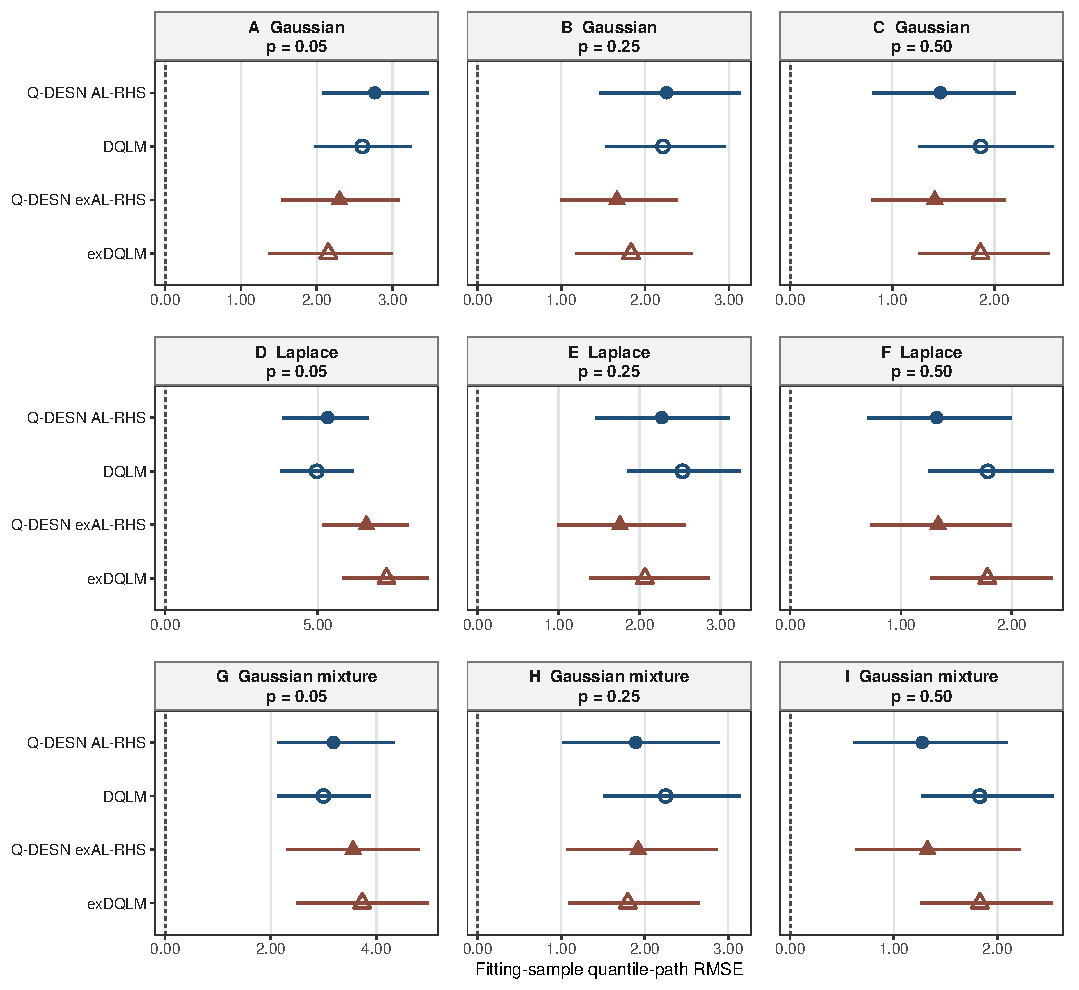
\includegraphics[width=0.98\textwidth]{figures/ch04-qdesn/independent_simulation/qdesn_validation_500obs_v14_mcmc_fit_rmse_intervals.pdf}
\caption[MCMC and variational fitting-sample recovery]{MCMC and variational
fitting-sample recovery in the single-quantile simulation, part I: MCMC.
Points are posterior means of quantile-path root mean squared error (RMSE) and
horizontal segments are equal-tailed 95\% posterior intervals; lower values
are better. Navy circles identify the \(\AL\) models and muted-brick triangles
the \(\exAL\) models; filled symbols denote Q--DESN and open symbols the
corresponding dynamic quantile linear model. Panels A--I identify the
data-generating family and probability level and use separate horizontal
scales. The dashed line marks exact recovery of the known conditional quantile
path. Intervals condition on the simulated series and case-specific selected
specification. Part II on the following page gives the corresponding
variational summaries, which are approximate and may use separately selected
specifications.}
\figalt{Nine panels compare posterior fitting-sample quantile-path RMSE means
and 95 percent intervals for four models across three innovation families and
three probability levels. Lower values are better.}
\label{qdesn:fig:simulation-500obs-fit-recovery-thesis}
\end{figure}

\begin{figure}[p]
\ContinuedFloat
\centering
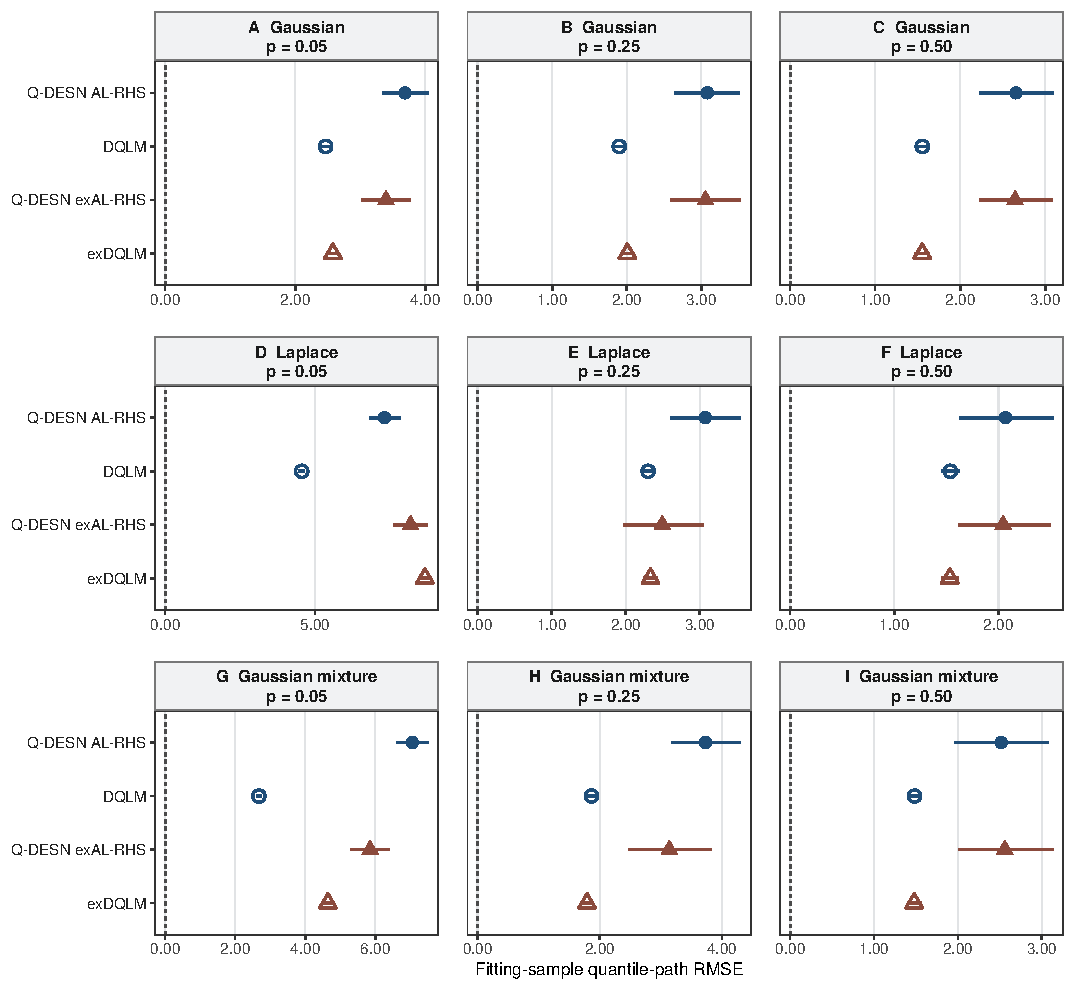
\includegraphics[width=0.98\textwidth]{figures/ch04-qdesn/independent_simulation/qdesn_validation_500obs_v14_vb_fit_rmse_intervals.pdf}
\caption*{Figure~\thefigure\ (continued), part II: variational fitting-sample
recovery in the single-quantile simulation. Points are variational posterior
means of quantile-path RMSE and horizontal segments are equal-tailed
approximate 95\% variational posterior intervals; lower values are better.
Model encodings and panels are as in part I. These intervals summarize the
variational approximation and condition on the simulated series, evaluation
design, and case-specific selected specification.}
\figalt{Nine panels compare approximate variational fitting-sample
quantile-path RMSE means and 95 percent intervals for four models across three
innovation families and three probability levels. Lower values are better.}
\end{figure}


\subsection{Single-quantile computation and diagnostics}
\label{qdesn:subsec:supp-independent-exal-mcmc-details}

The independent Q--DESN exAL--RHS MCMC analysis uses the mixture representation
for \(v\) described earlier in the technical development and an analysis-specific
scale-collapsed transition. Conditional on the remaining unknowns, the scale is
integrated from the conditional density used to update the asymmetry parameter
on a logit transformation of its bounded support, and the scale is then drawn
from its full conditional distribution. This transition is used for the
independent simulation analysis; Algorithm~\ref{qdesn:alg:qdesn_mcmc} gives the generic joint or
conditionally split update. The resulting draws determine the fitted and
forecast quantile paths used in the reported criteria.

The exDQLM baseline uses version 1.1.1 of the CRAN package \pkg{exdqlm}
\citep{qdesn-exdqlmRPackage}. For unrestricted exAL
fits, its MCMC sampler updates the asymmetry parameter from its conditional
distribution with the scale analytically integrated out, then draws the scale
from its full conditional distribution. Its variational calculation uses the
structured factorization \(q(\gamma)q(\sigma\mid\gamma)\). These model-specific
computations produce the
quantile-path draws evaluated by the common criteria above.
For retained pairs \((\sigma_b,\gamma_b)\),
\(b=1,\ldots,B_{\mathrm{post}}\), let
\begin{align*}
m_{\varepsilon,b}
&=\sigma_b\{A_p(\gamma_b)+D_p(\gamma_b)\sqrt{2/\pi}\},\\
V_{\varepsilon,b}
&=\sigma_b^2\{B_p(\gamma_b)+A_p(\gamma_b)^2
  +D_p(\gamma_b)^2(1-2/\pi)\}.
\end{align*}
The rolling-origin filter uses
\(\bar m_\varepsilon=B_{\mathrm{post}}^{-1}\sum_b m_{\varepsilon,b}\) and
\(\bar V_\varepsilon=B_{\mathrm{post}}^{-1}
\sum_b(V_{\varepsilon,b}+m_{\varepsilon,b}^2)-\bar m_\varepsilon^2\).
The parameter posterior from the initial fit is retained, while observations
available at successive origins update the state filter before forecasts are
propagated over the requested horizons.

The MCMC metric distributions generally pool 12,000 retained evaluations from
three independently initialized chains. The Q--DESN AL--RHS Gaussian
\(p=0.05\) forecast MAE and check-loss summaries use 3,000 retained evaluations
from three chains. Diagnostics assess between-chain agreement for each
draw-wise criterion.


\subsection{Single-quantile five-chain point-path sensitivity}
\label{qdesn:subsec:supp-independent-five-chain-sensitivity}

The primary single-quantile MCMC tables report draw-wise posterior summaries of
the evaluation criteria. The analysis below instead evaluates each criterion
on a posterior point estimate of the quantile path and provides a separate
sensitivity analysis across independently initialized chains.
For the Gaussian \(p=0.25\) comparison, a five-chain sensitivity analysis uses
five independently seeded chains for each model specification. For each chain,
the posterior point path is computed first; the reported sensitivity path is the
coordinatewise median of those five paths. All criteria are then recomputed
from that path. This construction summarizes chain-specific point estimates.

One common specification is reported for each working likelihood. Relative to
the corresponding criterion-specific summary, the \(\AL\)--\(\RHS\)
specification reduced fit RMSE by 8.4\% and forecast MAE by 1.6\%, while its
forecast check loss increased by 0.4\%. The \(\exAL\)--\(\RHS\) specification
reduced fit RMSE by 18.3\%, forecast MAE by 8.7\%, and forecast check loss by
0.4\%. Within the Gaussian \(p=0.25\) comparison, these results indicate
limited sensitivity to MCMC initialization for the selected specifications.

\subsection{Joint multi-quantile MCMC evaluation details}

The corrected shared-backbone evaluation uses the initialization sequence in
Figure~\ref{qdesn:fig:supp-quantile-sequential-initialization}. One scenario-specific
DESN/RHS specification is selected from source realizations and held common
across the four model classes. The evaluation realization is used only for the final
fit and evaluation. Table~\ref{qdesn:tab:joint-qdesn-corrected-v4-protocol}
records the 136 variational components, 160 MCMC chains, and retained-draw
allocation. All five chains within a model cell share fixed prior
hyperparameters and one posterior target; chain-specific dispersion affects
initial states only.

\begin{table}[p]
\centering
\scriptsize
\setlength{\tabcolsep}{3.7pt}
\renewcommand{\arraystretch}{1.04}
\resizebox{\textwidth}{!}{%
\begin{tabular}{@{}>{\raggedright\arraybackslash}p{0.20\textwidth}>{\raggedright\arraybackslash}p{0.30\textwidth}rrc@{}}
\toprule
Simulation setting & Model & Posterior mean & Median & Equal-tailed 95\% interval \\
\midrule
Asymmetric-Laplace tail & Joint Q--DESN \(\AL\)--\(\RHS\) & 0.7816 & 0.7583 & [0.3733, 1.3333] \\
 & Independent Q--DESN \(\AL\)--\(\RHS\) & 0.3553 & 0.3510 & [0.3305, 0.4085] \\
 & Joint exQDESN \(\exAL\)--\(\RHS\) & 0.4787 & 0.4202 & [0.3325, 0.9059] \\
 & Independent exQDESN \(\exAL\)--\(\RHS\) & \textbf{0.3324} & 0.3307 & [0.3212, 0.3518] \\
\addlinespace[2pt]
Gaussian-mixture innovations & Joint Q--DESN \(\AL\)--\(\RHS\) & 0.6019 & 0.5855 & [0.4362, 0.8648] \\
 & Independent Q--DESN \(\AL\)--\(\RHS\) & 0.3975 & 0.3967 & [0.3902, 0.4094] \\
 & Joint exQDESN \(\exAL\)--\(\RHS\) & 0.4261 & 0.4130 & [0.3902, 0.5310] \\
 & Independent exQDESN \(\exAL\)--\(\RHS\) & \textbf{0.3936} & 0.3926 & [0.3871, 0.4055] \\
\addlinespace[2pt]
Laplace innovations & Joint Q--DESN \(\AL\)--\(\RHS\) & 0.3856 & 0.3817 & [0.3472, 0.4441] \\
 & Independent Q--DESN \(\AL\)--\(\RHS\) & 0.3478 & 0.3460 & [0.3320, 0.3754] \\
 & Joint exQDESN \(\exAL\)--\(\RHS\) & \textbf{0.3335} & 0.3318 & [0.3246, 0.3525] \\
 & Independent exQDESN \(\exAL\)--\(\RHS\) & 0.3349 & 0.3334 & [0.3257, 0.3524] \\
\addlinespace[2pt]
Nonlinear reservoir dynamics & Joint Q--DESN \(\AL\)--\(\RHS\) & 0.4743 & 0.4724 & [0.4386, 0.5192] \\
 & Independent Q--DESN \(\AL\)--\(\RHS\) & 0.4317 & 0.4314 & [0.4271, 0.4384] \\
 & Joint exQDESN \(\exAL\)--\(\RHS\) & 0.4457 & 0.4438 & [0.4311, 0.4712] \\
 & Independent exQDESN \(\exAL\)--\(\RHS\) & \textbf{0.4296} & 0.4292 & [0.4253, 0.4362] \\
\addlinespace[2pt]
Gaussian innovations & Joint Q--DESN \(\AL\)--\(\RHS\) & 0.3539 & 0.3504 & [0.3243, 0.4028] \\
 & Independent Q--DESN \(\AL\)--\(\RHS\) & 0.3488 & 0.3461 & [0.3221, 0.3903] \\
 & Joint exQDESN \(\exAL\)--\(\RHS\) & 0.3331 & 0.3279 & [0.3116, 0.3851] \\
 & Independent exQDESN \(\exAL\)--\(\RHS\) & \textbf{0.3323} & 0.3299 & [0.3146, 0.3646] \\
\addlinespace[2pt]
Persistent heavy tails & Joint Q--DESN \(\AL\)--\(\RHS\) & 0.3837 & 0.3752 & [0.3636, 0.4507] \\
 & Independent Q--DESN \(\AL\)--\(\RHS\) & 0.3743 & 0.3729 & [0.3649, 0.3927] \\
 & Joint exQDESN \(\exAL\)--\(\RHS\) & 0.3867 & 0.3807 & [0.3639, 0.4485] \\
 & Independent exQDESN \(\exAL\)--\(\RHS\) & \textbf{0.3707} & 0.3691 & [0.3622, 0.3878] \\
\addlinespace[2pt]
Regime shift & Joint Q--DESN \(\AL\)--\(\RHS\) & 0.4349 & 0.4325 & [0.4256, 0.4570] \\
 & Independent Q--DESN \(\AL\)--\(\RHS\) & 0.4311 & 0.4298 & [0.4262, 0.4430] \\
 & Joint exQDESN \(\exAL\)--\(\RHS\) & 0.4398 & 0.4373 & [0.4266, 0.4654] \\
 & Independent exQDESN \(\exAL\)--\(\RHS\) & \textbf{0.4310} & 0.4301 & [0.4263, 0.4415] \\
\addlinespace[2pt]
Student-\(t\) location--scale & Joint Q--DESN \(\AL\)--\(\RHS\) & 0.3795 & 0.3646 & [0.3425, 0.4964] \\
 & Independent Q--DESN \(\AL\)--\(\RHS\) & 0.3603 & 0.3582 & [0.3451, 0.3886] \\
 & Joint exQDESN \(\exAL\)--\(\RHS\) & 0.3695 & 0.3576 & [0.3405, 0.4607] \\
 & Independent exQDESN \(\exAL\)--\(\RHS\) & \textbf{0.3521} & 0.3502 & [0.3408, 0.3747] \\
\bottomrule
\end{tabular}
}%
\caption{Corrected posterior DGP-integrated \(\aCRPS\) for the joint multi-quantile study. Entries are posterior means, medians, and equal-tailed 95\% intervals. Boldface marks the lowest posterior mean within each simulation setting. All winner/runner-up marginal intervals overlap, so the rankings are descriptive. Crossing frequencies and the sizes of the monotone adjustments are reported separately.}
\label{qdesn:tab:joint-qdesn-corrected-v4-score}
\end{table}


Figure~\ref{qdesn:fig:joint-qdesn-corrected-v4-fit-rmse} compares
fitting-sample recovery under the same shared feature design used for the
forecast-score comparison above.

\begin{figure}[!htbp]
\centering
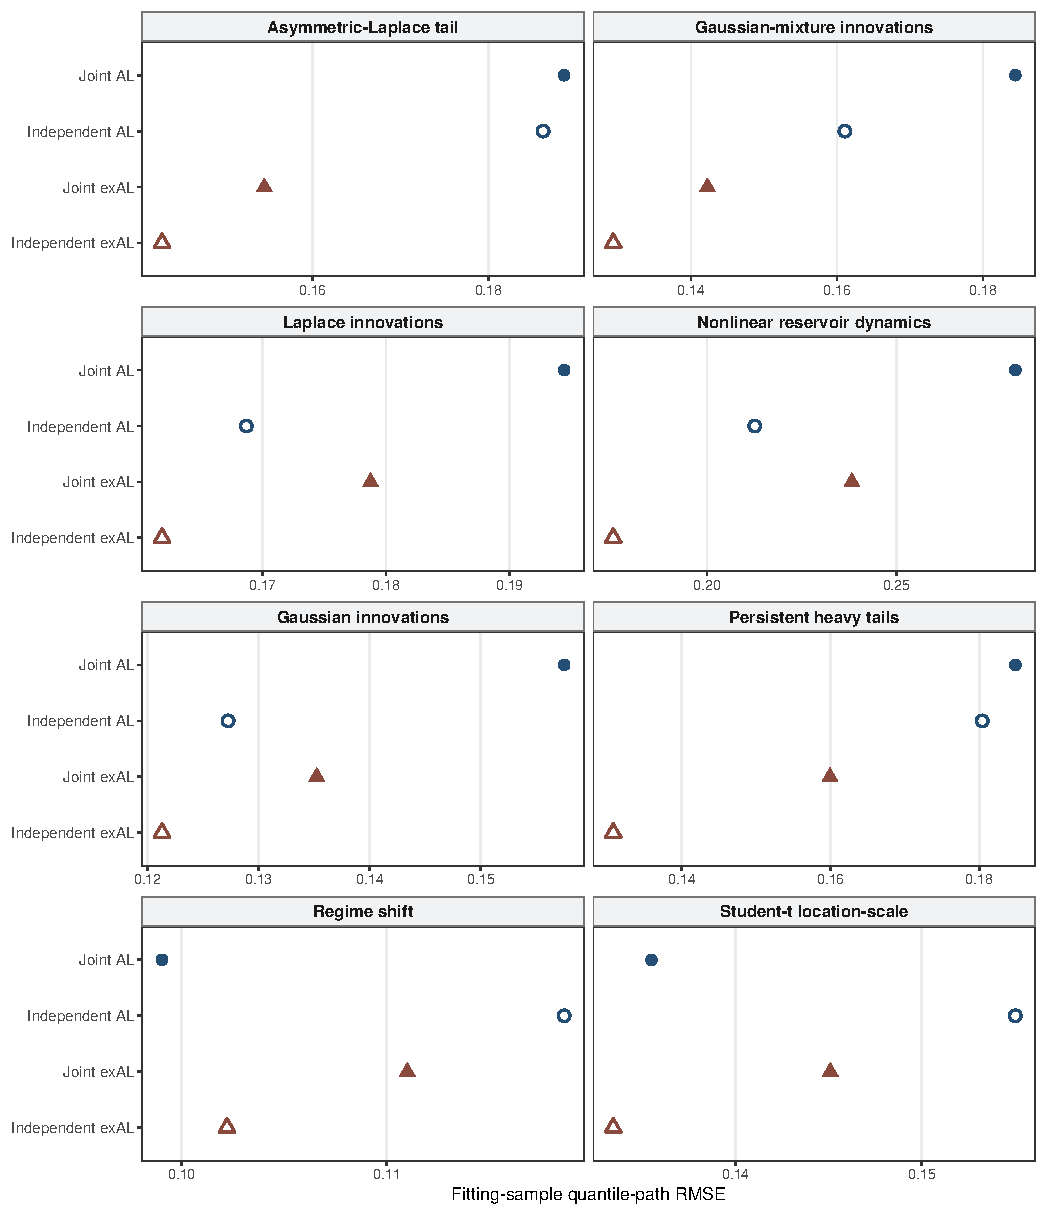
\includegraphics[width=0.94\textwidth]{figures/ch04-qdesn/joint_qdesn_simulation/joint_qdesn_corrected_v4_fit_oracle_rmse.pdf}
\caption{Fitting-sample recovery of the known conditional quantile paths in the corrected joint study. Points are RMSE values for the reported posterior-mean quantile grids, not posterior intervals. Filled symbols denote joint fits, open symbols independent fits, blue \(\AL\), and red \(\exAL\). Crossing frequencies and monotone-adjustment magnitudes are reported separately.}
\label{qdesn:fig:joint-qdesn-corrected-v4-fit-rmse}
\end{figure}


The posterior-score diagnostics satisfy the pre-specified rank-normalized
\(\widehat R\), effective-sample-size, and Monte Carlo error criteria in 22 of
32 comparisons; the other 10 are retained with review status. All 16
\(\exAL\) scale--asymmetry assessments are also retained at review level.
The least favorable joint nonlinear-reservoir assessment has gamma
rank-normalized \(\widehat R=1.125\) and bulk effective sample size 41.7.
Precision stabilization was invoked in 26 joint chains for 159 coefficient
updates; the maximum relative diagonal perturbation was \(10^{-12}\), below
the pre-specified \(10^{-8}\) failure threshold. All repaired chains satisfy
the numerical checks and no result is excluded on this basis.

Four paired joint-minus-independent score intervals lie entirely above zero,
favoring independent estimation, and the other twelve include zero. Raw
crossing rates and monotone-adjustment magnitudes are reported separately from
the score after rearrangement. All posterior-mean grids are ordered after
rearrangement.

\begin{table}[!htbp]
\centering
\scriptsize
\begin{tabular}{@{}>{\raggedright\arraybackslash}p{0.25\textwidth}>{\raggedright\arraybackslash}p{0.65\textwidth}@{}}
\toprule
Item & Specification \\
\midrule
Feature design & One scenario-specific DESN/RHS specification is selected on separate source realizations and shared by all four model classes; the evaluation realization is excluded from selection. \\
Quantile grid & 0.05, 0.10, 0.25, 0.50, 0.75, 0.90, and 0.95. \\
Sequential initialization & Gaussian ridge initializes Gaussian RHS--VB; independent AL fits proceed outward from the median; each AL fit initializes exAL at the same level; complete independent grids initialize the corresponding joint fits; matching VB fits initialize MCMC. \\
Common posterior target & All five chains in a model cell share fixed prior hyperparameters and one verified posterior-target hash. Dispersed initial states do not enter prior centers. The RHS global-scale shape uses \((d_\beta+1)/2\). \\
Posterior simulation & Five chains per model cell. AL chains use 4,000 iterations, 1,000 burn-in iterations, and thinning by four; exAL chains use 8,000 iterations, 2,000 burn-in iterations, and thinning by four. The complete calculation retains 180,000 draws. \\
Score distribution & The primary summary uses 750 equally spaced retained draws from each chain, or 3,750 chain-balanced draws per model cell. Independent quantile draws use the pre-specified seeded product coupling; joint draws preserve cross-level identity. \\
Forecast evaluation & Each comparison uses the same 990 sequentially conditional origin--horizon rows. The primary criterion is DGP-integrated \(\aCRPS\) after monotone reporting. \\
\bottomrule
\end{tabular}
\caption{Design of the corrected common-posterior joint multi-quantile evaluation. Initialization transfers starting values only; each destination retains its own likelihood, prior, and posterior target.}
\label{qdesn:tab:joint-qdesn-corrected-v4-protocol}
\end{table}

\begin{table}[!htbp]
\centering
\scriptsize
\begin{tabular}{@{}>{\raggedright\arraybackslash}p{0.39\textwidth}rr@{}}
\toprule
Simulation setting & \(\AL\) & \(\exAL\) \\
\midrule
Asymmetric-Laplace tail & \textbf{0.4263 [0.0184, 0.9880]} & 0.1463 [-0.0037, 0.5677] \\
Gaussian-mixture innovations & \textbf{0.2044 [0.0368, 0.4678]} & 0.0325 [-0.0060, 0.1397] \\
Laplace innovations & 0.0378 [-0.0094, 0.0995] & -0.0014 [-0.0217, 0.0199] \\
Nonlinear reservoir dynamics & \textbf{0.0426 [0.0056, 0.0881]} & \textbf{0.0161 [0.0002, 0.0421]} \\
Gaussian innovations & 0.0052 [-0.0482, 0.0619] & 0.0008 [-0.0394, 0.0558] \\
Persistent heavy tails & 0.0094 [-0.0204, 0.0772] & 0.0160 [-0.0142, 0.0787] \\
Regime shift & 0.0038 [-0.0126, 0.0266] & 0.0087 [-0.0085, 0.0351] \\
Student-\(t\) location--scale & 0.0192 [-0.0314, 0.1379] & 0.0174 [-0.0224, 0.1089] \\
\bottomrule
\end{tabular}
\caption{Joint-minus-independent contrasts in posterior DGP-integrated \(\aCRPS\). Entries are posterior means with equal-tailed 95\% intervals under the pre-specified chain-balanced pairing. Positive values favor independent estimation. Boldface marks the four intervals lying entirely above zero; the other twelve include zero, and none favors joint estimation.}
\label{qdesn:tab:supp-joint-qdesn-corrected-v4-contrasts}
\end{table}

\begin{table}[!htbp]
\centering
\scriptsize
\setlength{\tabcolsep}{3.5pt}
\resizebox{\textwidth}{!}{%
\begin{tabular}{@{}>{\raggedright\arraybackslash}p{0.31\textwidth}rrrr@{}}
\toprule
Model & \shortstack{Fit raw crossings\\rate (count/\(N\))} & \shortstack{Fit adjustment\\mean/max} & \shortstack{Forecast raw crossings\\rate (count/\(N\))} & \shortstack{Forecast adjustment\\mean/max} \\
\midrule
Joint Q--DESN \(\AL\)--\(\RHS\) & 0.09\% (21/24,000) & 0.0000/0.0813 & 2.52\% (1,197/47,520) & 0.0118/0.6949 \\
Independent Q--DESN \(\AL\)--\(\RHS\) & 0.47\% (114/24,000) & 0.0003/0.1845 & 7.41\% (3,522/47,520) & 0.0166/0.7034 \\
Joint exQDESN \(\exAL\)--\(\RHS\) & 0.00\% (0/24,000) & 0.0000/0.0000 & 0.00\% (0/47,520) & 0.0000/0.0000 \\
Independent exQDESN \(\exAL\)--\(\RHS\) & 0.00\% (0/24,000) & 0.0000/0.0000 & 0.57\% (269/47,520) & 0.0005/0.1887 \\
\bottomrule
\end{tabular}
}%
\caption{Frequency and magnitude of monotone correction for the posterior-mean quantile grids, aggregated over eight simulation settings. Crossing rates are the proportions of adjacent-level comparisons that cross before rearrangement; counts and total opportunities \(N\) are shown in parentheses. Adjustment entries give the mean and maximum absolute change on the simulation response scale induced by the pre-specified monotone rule. Thus the rates measure how often crossings occur, whereas the adjustment summaries describe their magnitude. All rearranged grids have zero crossings.}
\label{qdesn:tab:supp-joint-qdesn-corrected-v4-crossings}
\end{table}


The secondary realized-outcome score and oracle-recovery tables in the source
baseline do not alter the primary known-DGP score conclusion. Independent
exQDESN has the smallest secondary realized-outcome score in seven of eight
mechanisms, with joint exQDESN smallest for the Laplace mechanism. For forecast
quantile-path recovery, independent exQDESN has the smallest MAE in seven
mechanisms and independent Q--DESN in the regime-shift mechanism. These are
point-path diagnostics, not posterior proper-score comparisons against new
realized responses.

This comparison replaces the earlier provisional packet in full. If
\(d_\beta\) denotes the number of penalized coefficients in an RHS
global-scale block, the corrected calculation uses shape
\((d_\beta+1)/2\). Prior centers and hyperparameters are fixed within each
model cell and do not depend on dispersed chain-specific starting values.
Posterior-target hashes agree across all five chains in each of the 32 model
cells. The replacement is based on the common posterior target; no cell was
selected according to whether its corrected score improved.

The separate 50-replicate variational sensitivity gives negative paired
\(\AL\)-minus-\(\exAL\) forecast-MAE differences for both joint and independent
fits in every mechanism. The proportions favoring AL range from 70\% to 100\%
for joint fits and from 82\% to 96\% for independent fits. This sensitivity
concerns approximate quantile-path MAE; the MCMC DGP-integrated score remains
the primary ranking criterion.

% migration-id: MIG-CH04-05
\section{Latent-path ensemble-likelihood construction}
\label{qdesn:sec:glofas_discrepancy}

\noindent\textbf{Model overview.}
The streamflow application combines the historical and issued Global Flood
Awareness System (GloFAS) products with a reference gauge record
\citep{qdesn-AlfieriEtAl2013GloFAS,qdesn-HarriganEtAl2023GloFASForecasts}. Separate DESN
feature maps represent the reference process and the GloFAS-minus-reference
discrepancy. The selected Part 4 analysis is a joint AL--RHS variational fit:
post-cutoff reference values are latent during fitting, and the issued ensemble
contributes directly to the same latent-path analysis. It is not a post-fit
forecast adjustment.

\subsection{Observed quantities and latent design}
\label{qdesn:subsec:glofas_aug_design}

Let \(T\) denote 25~December~2022 and let
\(y_t=\log(y_t^{\mathrm{USGS}}+1)\) be transformed reference streamflow.
Write \(g_t^{\mathrm{ret}}\) for transformed retrospective GloFAS and
\(g_{T+h,e}^{\mathrm{ens}}\) for transformed issued member \(e\) at horizon
\(h\). The requested future path
\(\vect y_F=(y_{T+1},\ldots,y_{T+30})^\top\) is unobserved during fitting.
Issued GloFAS values are available for the first 28 horizons, with 51 members
at each horizon. The withheld USGS values are loaded only after fitting for
forecast evaluation. Realized PRISM/ERA5 precipitation and soil-moisture
covariates are used after \(T\), so the calculation is a retrospective
oracle-covariate diagnostic.

For probability level \(p_k\), the reference and discrepancy quantile
locations are
\begin{equation}
\begin{aligned}
\text{Reference quantile:}\quad
q_{k,t}
&=\vect x_t^{\mathrm{ref}\top}\vect\beta_k,\\
\text{Discrepancy quantile:}\quad
d_{k,t}
&=\vect x_t^{\mathrm{disc}\top}\vect\delta_k,\\
\text{GloFAS quantile:}\quad
q_{k,t}^{\mathrm{glo}}
&=q_{k,t}+d_{k,t}.
\end{aligned}
\label{qdesn:eq:supp_glofas_quantile_decomposition}
\end{equation}
Historical reference features are generated from the observed reference
history, and historical discrepancy features are generated from
\(g_t^{\mathrm{ret}}-y_t\). After \(T\), the reference and discrepancy
reservoir states are recomputed as functions of the latent path
\(\vect y_F\). Strict lagging is imposed: the design row for \(T+h\) may
depend on earlier latent values but not on \(y_{T+h}\).

For one probability level, stack the reference and discrepancy coefficients as
\[
\vect\theta_k=
\begin{bmatrix}\vect\beta_k\\ \vect\delta_k\end{bmatrix},
\qquad
\vect h_t^{\mathrm{ref}}=
\begin{bmatrix}\vect x_t^{\mathrm{ref}}\\ \vect 0\end{bmatrix},
\qquad
\vect h_t^{\mathrm{glo}}=
\begin{bmatrix}\vect x_t^{\mathrm{ref}}\\
\vect x_t^{\mathrm{disc}}\end{bmatrix}.
\]
Then \(\vect h_t^{\mathrm{ref}\top}\vect\theta_k=q_{k,t}\) and
\(\vect h_t^{\mathrm{glo}\top}\vect\theta_k=q_{k,t}+d_{k,t}\).
Conditional on \(\vect y_F\), these are ordinary fixed-design Q--DESN
regressions.

The selected reference reservoir has depth one, width
\(\GlofasApplicationCurrentReferenceReservoirSize{}\), memory
\(\GlofasApplicationCurrentReferenceReservoirMemory{}\), leak rate
\(\GlofasApplicationCurrentReferenceReservoirAlpha{}\), spectral radius
\(\GlofasApplicationCurrentReferenceReservoirRho{}\), washout
\(\GlofasApplicationCurrentReferenceReservoirWashout{}\), and seed
\(\GlofasApplicationCurrentReferenceReservoirSeed{}\). Its inputs are reference
lags 1--360 and realized precipitation and soil-moisture lags 0--180. The
discrepancy reservoir has width
\(\GlofasApplicationCurrentDiscrepancyReservoirSize{}\), memory
\(\GlofasApplicationCurrentDiscrepancyReservoirMemory{}\), leak rate
\(\GlofasApplicationCurrentDiscrepancyReservoirAlpha{}\), spectral radius
\(\GlofasApplicationCurrentDiscrepancyReservoirRho{}\), washout
\(\GlofasApplicationCurrentDiscrepancyReservoirWashout{}\), and seed
\(\GlofasApplicationCurrentDiscrepancyReservoirSeed{}\). It uses the
corresponding discrepancy and weather lags. Neither feature map includes
direct readout inputs. The reference and discrepancy RHS scales are
\(\tau_{0,\mathrm{ref}}=\GlofasApplicationCurrentSharedRhsTau{}\) and
\(\tau_{0,\mathrm{disc}}=\GlofasApplicationCurrentDiscrepancyRhsTau{}\).

\subsection{Weighted augmented working likelihood}
\label{qdesn:subsec:glofas_likelihoods}

At each level \(p_k\), reference observations have AL location \(q_{k,t}\),
whereas retrospective and issued GloFAS observations have location
\(q_{k,t}+d_{k,t}\). Let \(z_i^c\) and \(\vect h_i^c\) denote an observation
and design row from source \(c\in\{\mathrm{ref},\mathrm{glo}\}\). The AL
normal--exponential augmentation is
\begin{equation}
\begin{aligned}
\text{Latent scale:}\quad
v_{i,k}^c\mid\sigma_{c,k}
&\sim\Exp(\mathrm{rate}=1/\sigma_{c,k}),\\
\text{Conditional observation:}\quad
z_i^c\mid\cdot
&\sim\Normal\!\left(
\vect h_i^{c\top}\vect\theta_k+A_{0,k}v_{i,k}^c,\,
\sigma_{c,k}B_{0,k}v_{i,k}^c
\right).
\end{aligned}
\label{qdesn:eq:supp_glofas_al_hierarchy}
\end{equation}

Define an observation weight \(w_i=1\) for historical reference and
retrospective GloFAS rows. For an issued member at a fixed horizon,
\(w_i=1/51\). Hence the 51 issued members contribute total weight one at each
horizon. The executed augmented working likelihood has the form
\begin{equation}
\begin{aligned}
L_{\mathrm{aug}}(\Theta)
\ \propto\
\prod_{k=1}^{K}\prod_{c}\prod_{i\in\mathcal I_c}
\left[
p(z_i^c\mid v_{i,k}^c,\Theta_k)\,
p(v_{i,k}^c\mid\sigma_{c,k})
\right]^{w_i}.
\end{aligned}
\label{qdesn:eq:supp_glofas_weighted_augmented_likelihood}
\end{equation}
This is a complete-data fractional or power-likelihood construction. It
prevents the issued ensemble from receiving 51 times the weight of one
historical time point. Because the power is applied before integrating out the
latent variables, Eq.~\eqref{qdesn:eq:supp_glofas_weighted_augmented_likelihood} is
not asserted to be an exact fractional marginal AL posterior.

The source-specific scales, coefficient priors, and latent variables are
updated under this weighted augmentation. The exAL comparator additionally
contains source-specific shape parameters and positive-shift latent variables,
using the structured quadrature calculations described earlier. The selected
application result uses AL, not exAL.

\subsection{Joint quantile and latent-path approximation}
\label{qdesn:subsec:glofas_latent_path}

The fitted grid is
\[
(0.05,\ 0.20,\ 0.35,\ 0.50,\ 0.65,\ 0.80,\ 0.95).
\]
The seven reference coefficient blocks and seven discrepancy coefficient
blocks are linked by separate adjacent-quantile RHS priors. Computation uses
mean-field quantile-block coordinate updates initialized from the completed
independent fits. The construction shares information through these priors; it
is not a single exact Gaussian update over every coefficient and latent-path
block.

Let \(\ell_F(\vect y_F)\) be the expected weighted augmented log likelihood,
under the other current variational factors, for terms whose response or
design depends on \(\vect y_F\). At its mode
\(\widehat{\vect y}_F\), the latent-path factor is approximated by
\begin{equation}
\begin{aligned}
\text{Latent-path factor:}\quad
\mat K_F&=-\nabla^2\ell_F(\widehat{\vect y}_F),&
q_F(\vect y_F)&\approx
\Normal(\widehat{\vect y}_F,\mat K_F^{-1}).
\end{aligned}
\label{qdesn:eq:supp_glofas_future_path_factor}
\end{equation}
For design row \(\vect h_i^c(\vect y_F)\), let \(\mat J_i\) be its Jacobian at
the mode and \(\mat V_F=\mat K_F^{-1}\). The first-order moments propagated to
the remaining updates are
\begin{equation}
\begin{aligned}
\text{Propagated design moments:}\quad
\E\{\vect h_i^c(\vect y_F)\}
&\approx \vect a_i^c,\\
\E\{\vect h_i^c\vect h_i^{c\top}\}
&\approx \vect a_i^c\vect a_i^{c\top}
+\mat J_i\mat V_F\mat J_i^\top,
\end{aligned}
\label{qdesn:eq:supp_glofas_future_path_delta}
\end{equation}
where \(\vect a_i^c=\vect h_i^c(\widehat{\vect y}_F)\). The corresponding
Jacobian--covariance term is retained for cross-moments involving a component
of \(\vect y_F\). This gives a Laplace--Delta approximation to the nonlinear
latent-path objective. No separate forecast adapter, future-response
imputation from the withheld truth, or post-hoc crossing correction is used.

\subsection{Numerical qualification and sensitivity results}
\label{qdesn:subsec:glofas_checks}

The inherited 50-iteration RHS warmup corresponds to five joint outer sweeps
because every sweep contains at least ten inner coefficient iterations. The
retained source fit completed those five sweeps without a global-scale update.
The continuation preserved that fitted state, released the global scales at
sweep 6, and completed five post-release updates through sweep 10. All inner
fits converged, the RHS gate passed, and every one of the 14 reference and
discrepancy RHS blocks changed after release. The final maximum parameter
change was \(0.004153866\), exceeding the strict outer tolerance \(0.001\).
Accordingly, the selected Joint AL estimate is cap-stabilized after RHS
release, not strictly outer-converged. The optional Joint exAL continuation was
stopped; its source fit is retained only as a nonconverged sensitivity result.
No MCMC fit was used for this application.

On the original streamflow scale, Joint AL has \(\aCRPS=27.132\), median
MAE \(1.374\), and median RMSE \(1.531\), compared with \(39.401\), \(1.751\),
and \(1.919\) for raw GloFAS. These values supplement the transformed-scale
scores in Table~\ref{qdesn:tab:glofas-application-score}; they do not change
the single-origin or cap-stabilized qualifications. The Gaussian predictive
baselines are retained in that table rather than repeated as a secondary
figure because their low transformed-scale \(\aCRPS\) accompanies central
90\% coverage of only \(0.250\) and \(0.179\).

\begin{figure}[p]
\centering
\includegraphics[width=0.98\textwidth]{\GlofasApplicationCurrentIndependentComparisonFigure}
\caption[Independent and joint GloFAS sensitivity comparisons]{Independent and
joint GloFAS sensitivity comparisons, part I: independent AL and exAL quantile
regressions. Panels use the same dates, probability-level palette, and data
encoding as Figure~\ref{qdesn:fig:glofas-application-forecast-period}. Historical
quantile paths are dashed and issued paths are solid. Panel strips report the
forecast-window \(\aCRPS\) and empirical coverage of the central 90\% interval.
Part II on the following page gives the joint sensitivity comparison.}
\figalt{Paired panels compare independent AL and exAL quantile paths before and
after the forecast origin. Observed USGS values use filled green circles,
withheld values use open green circles, and GloFAS values are orange.}
\label{qdesn:fig:supp-glofas-part4-independent-comparison}
\end{figure}

\begin{figure}[p]
\ContinuedFloat
\centering
\includegraphics[width=0.98\textwidth]{\GlofasApplicationCurrentJointComparisonFigure}
\caption*{Figure~\thefigure\ (continued), part II: joint AL and exAL quantile
regressions for the GloFAS application.
Joint AL is the selected fit. Joint exAL is shown only as a sensitivity result
because its source fit did not satisfy the numerical qualification rule. The
common encoding and forecast-window summaries permit a descriptive comparison
without treating the Joint exAL result as an eligible selection candidate.}
\figalt{Paired panels compare selected Joint AL quantile paths with unqualified
Joint exAL sensitivity paths over common historical and forecast dates. A
vertical line marks the forecast origin.}
\end{figure}

Removing the GloFAS source and discrepancy coefficients recovers the ordinary
Q--DESN regression. Holding the future path fixed recovers the fixed-design
updates. Strict forecast lagging, the future-truth firewall, source indexing,
horizon weights, RHS release certificate, and agreement between the stored and
reconstructed score summaries provide implementation checks. Posterior
calibration beyond this single origin remains an empirical question.

% migration-id: MIG-CH04-06
\section{Regional heterogeneity and historical sensitivity}
\label{qdesn:subsec:supp_pricefm_diagnostics}

The principal results above report the complete 114-case PriceFM comparison under the
region-frozen protocol. For each region, the training- and validation-selected
Q--DESN specification is held fixed across all three test folds. The complete
registry contains no post-test changes and no case-level fallback to the
earlier R92 surface.

R98 has mean AQL 7.217, compared with 7.039 for PriceFM. Q--DESN is lower in
54 of 114 region--fold comparisons and in 16 of 38 region means. The fold-level
contrast changes sign: Q--DESN is slightly lower in fold~2, while PriceFM is
lower in folds~1 and 3. This variation is more informative than the aggregate
alone, but it does not alter the primary conclusion that R98 has slightly
higher overall AQL. The deprecated R92 surface has mean AQL 6.824; it is a
historical sensitivity result under a held-out-informed selection rule, not a
fallback or part of the R98 estimate. The former 72-case forecast-lead summary
is not reproduced because it is not a complete R98 horizon analysis.

\begin{figure}[!htbp]
\centering
\includegraphics[width=\textwidth]{\PricefmCurrentRegionFigure}
\caption{Mean AQL across the three test folds for each PriceFM region. Blue
squares show the prospectively frozen R98 Q--DESN specification, green circles
show the matched PriceFM forecasts, and gray crosses show the deprecated R92
surface as historical sensitivity only. Regions are ordered by increasing R98
mean AQL; lower values are better.}
\figalt{For each of 38 regions, the plot compares mean AQL across three folds
for R98 Q--DESN, PriceFM, and historical R92 Q--DESN. The horizontal positions
show substantial regional heterogeneity, with PriceFM lower in 22 region means
and R98 Q--DESN lower in 16.}
\label{qdesn:fig:supp-pricefm-r98-region-comparison}
\end{figure}
